\documentclass[10pt,spanish,Letterpaper,openany]{book}
\usepackage{lmodern}
\usepackage{setspace}
\setstretch{0.95}
\usepackage{amssymb,amsmath}
\usepackage{ifxetex,ifluatex}
\usepackage{fixltx2e} % provides \textsubscript
\ifnum 0\ifxetex 1\fi\ifluatex 1\fi=0 % if pdftex
  \usepackage[T1]{fontenc}
  \usepackage[utf8]{inputenc}
\else % if luatex or xelatex
  \ifxetex
    \usepackage{mathspec}
  \else
    \usepackage{fontspec}
  \fi
  \defaultfontfeatures{Ligatures=TeX,Scale=MatchLowercase}
    \setmainfont[Scale=1.0]{Palatino Linotype}
    \setsansfont[]{Corbel}
    \setmonofont[Mapping=tex-ansi]{Corbel}
\fi

\makeatletter
\renewcommand\mainmatter{\clearpage\@mainmattertrue\pagenumbering{arabic}}
\renewcommand\frontmatter{\clearpage\@mainmatterfalse\pagenumbering{arabic}}
\renewcommand\backmatter{\clearpage\@mainmatterfalse}
\makeatother

%\usepackage{etoolbox}
%\makeatletter
%\patchcmd{\@smemmain}{\cleardoublepage}{\clearpage}{}{}
%\patchcmd{\@smemmain}{\cleardoublepage}{\clearpage}{}{}
%\patchcmd{\@smemfront}{\cleardoublepage}{\clearpage}{}{}
%\patchcmd{\@smemfront}{\cleardoublepage}{\clearpage}{}{}
%\makeatother

\setlength{\parindent}{0em}

\usepackage{graphicx}
\usepackage{booktabs}
\usepackage{multicol}
\usepackage{doc}
\usepackage{float}
\usepackage{tcolorbox} 
\usepackage{lipsum}
\usepackage{tikz}
\usepackage{nonfloat}

\usepackage{pdfpages}

\usepackage[
contents={},
opacity=1,
scale=1.5,
color=blue!90
]{background}
\usepackage{lipsum}
\usepackage{ifthen}

\usepackage{xcolor}
\usepackage[pagestyles]{titlesec}

\setlength{\footskip}{4mm}

\newcommand{\circledpage}{%
  \textcolor{colorlinetitle}{\rule[0.5ex]{0.8cm}{0.5pt}\enspace\thepage\enspace\rule[0.5ex]{0.8cm}{0.5pt}}%
}

\renewpagestyle{plain}[\normalsize\sffamily\bfseries\slshape]{
  \setfoot{}{\circledpage}{}}

\newpagestyle{myps}[\normalsize\sffamily\bfseries\slshape]{
  \setfoot{}{\circledpage}{}}

\pagestyle{myps}


\usepackage{framed}
\definecolor{colorlinetitle}{HTML}{a87e00}%{a87e00}%
\definecolor{naranja}{HTML}{D4AF37}%
\definecolor{textlinetitle}{HTML}{061769}%{061769}%{061769}%
\definecolor{fondo}{HTML}{041d57}%
\definecolor{newfondo}{HTML}{3d0718}%
\colorlet{shadecolor}{fondo!81!}


% use upquote if available, for straight quotes in verbatim environments
\IfFileExists{upquote.sty}{\usepackage{upquote}}{}
% use microtype if available
\IfFileExists{microtype.sty}{%
\usepackage{microtype}
\UseMicrotypeSet[protrusion]{basicmath} % disable protrusion for tt fonts
}{}
\usepackage[inner=12.7mm,outer=10mm,top=23mm,bottom=18.5mm]{geometry}
\PassOptionsToPackage{hyphens}{url}
\usepackage{hyperref}
\hypersetup{unicode=true,
            pdfborder={0 0 0},
            breaklinks=true}
\urlstyle{same}  % don't use monospace font for urls
\ifnum 0\ifxetex 1\fi\ifluatex 1\fi=0 % if pdftex
  \usepackage[shorthands=off,main=spanish]{babel}
\else
  \usepackage{polyglossia}
    % Fallback por si no viene definido desde Pandoc
  \setmainlanguage{spanish}
\fi
\usepackage{natbib}
\bibliographystyle{plainnat}
\usepackage{longtable,booktabs}
\IfFileExists{parskip.sty}{%
\usepackage{parskip}
}{% else
\setlength{\parindent}{0pt}
\setlength{\parskip}{6pt plus 2pt minus 1pt}
}
\setlength{\emergencystretch}{5em}  % prevent overfull lines
\providecommand{\tightlist}{%
  \setlength{\itemsep}{0pt}\setlength{\parskip}{0pt}}
\setcounter{secnumdepth}{5}
% Redefines (sub)paragraphs to behave more like sections
\ifx\paragraph\undefined\else
\let\oldparagraph\paragraph
\renewcommand{\paragraph}[1]{\oldparagraph{#1}\mbox{}}
\fi
\ifx\subparagraph\undefined\else
\let\oldsubparagraph\subparagraph
\renewcommand{\subparagraph}[1]{\oldsubparagraph{#1}\mbox{}}
\fi

%%% Use protect on footnotes to avoid problems with footnotes in titles
\let\rmarkdownfootnote\footnote%
\def\footnote{\protect\rmarkdownfootnote}


  \title{}
    \author{}
    \date{}
  
% no title page
\AtBeginDocument{\let\maketitle\relax}

% === Fuente para títulos ===
\newfontfamily\playfairfont{Playfair Display}[BoldFont=Playfair Display Bold, ItalicFont=Playfair Display Italic]

% === Color de títulos (azul etiquetas) ===
\definecolor{textlinetitle}{HTML}{152750}

% === Negrita en azul (preguntas entrevista, palabras clave, subtítulos) ===
\let\origtextbf\textbf
\renewcommand{\textbf}[1]{{\color{textlinetitle}\origtextbf{#1}}}

% === Interruptor para suprimir completamente el título de capítulo en artículos ===
% Usar \suppresschaptertrue  al inicio de cada artículo (en bloque {=latex})
% Usar \suppresschapterfalse para prefacios/secciones donde sí se quiere título
\newif\ifsuppresschapter
\suppresschapterfalse  % por defecto: comportamiento normal

% === Flag: indica que \includepdf ya hizo el salto de página ===
% Activar con \afterpdftrue justo después de cada \includepdf de sección
% Se desactiva automáticamente tras el primer \clearpage
\newif\ifafterpdf
\afterpdffalse

% === Flag para suprimir el cintillo en portadas y contraportada ===
\newif\ifsuppressbackground
\suppressbackgroundfalse

% === Suprimir capítulos sin título (portadas de sección) en PDF ===
% Cuando el título del capítulo está vacío, no imprime nada
% Cuando \suppresschaptertrue está activo, tampoco imprime ni el espacio
\makeatletter

\let\orig@makechapterhead\@makechapterhead
\renewcommand{\@makechapterhead}[1]{%
  \ifsuppresschapter
    \ifafterpdf
      \afterpdffalse  % consumir flag
    \else
      \clearpage
    \fi
  \else
    \orig@makechapterhead{#1}%
  \fi
}
\renewcommand{\@makeschapterhead}[1]{%
  \ifsuppresschapter
    % No imprime nada, ni espacio
  \else
    \ifdim\wd\@tempboxa=0pt\relax
    \else
      \vspace*{10\p@}%
      {\parindent \z@ \raggedright
        \normalfont
        \interlinepenalty\@M
        \Huge \bfseries #1\par\nobreak
        \vskip 20\p@
      }%
    \fi
  \fi
}
\makeatother


% === Secciones automáticas ===
\usepackage{pdfpages}    % ya lo usas
\usepackage{ifthen}      % ya lo usas
\usepackage{background}  % ya lo usas


% Macro: \SectionPDF{<path/pdf>}{<pagina_limite>}
% Muestra el PDF de la sección e impone el fondo hasta "pagina_limite-1"
\newcommand{\SectionPDF}[2]{%
  % Incrusta el PDF completo de la sección
  \includepdf[pages=-]{#1}%
  % Aplica fondo en cada página hasta el límite indicado
  \AddEverypageHook{%
    \ifthenelse{\value{page}<#2}{%
      \ifthenelse{\isodd{\value{page}}}{%
        \backgroundsetup{scale=1, color=white, opacity=1, angle=0, contents={%
          
\includegraphics[width=\paperwidth,height=\paperheight]{latex/background_numberimpar.pdf}}}%
      }{%
        \backgroundsetup{scale=1, color=white, opacity=1, angle=0, contents={%
          
\includegraphics[width=\paperwidth,height=\paperheight]{latex/background_numberpar.pdf}}}%
      }%
    }{}%
    \BgMaterial
  }%
}


\usepackage{caption2}
\captionsetup{%
labelsep=colon,%
font={footnotesize},%
aboveskip=0.4\baselineskip,%
belowskip=0\baselineskip,% deve essere 0 perché regolo lo spazio dal testo con \intextsep
}%

\usepackage{booktabs}
\usepackage{longtable}

% === Fix para tablas de 3+ columnas generadas por pandoc ===
\usepackage{array}
\usepackage{calc}
\newcommand{\real}[1]{#1}

\usepackage{indentfirst}
\setlength{\parindent}{1em}
\usepackage{enumitem}
\setlist[itemize]{labelindent = \parindent, leftmargin=*}

%\usepackage{framed,color}
%\definecolor{shadecolor}{RGB}{248,248,248}

\renewcommand{\textfraction}{0.05}
\renewcommand{\topfraction}{0.8}
\renewcommand{\bottomfraction}{0.8}
\renewcommand{\floatpagefraction}{0.75}

\renewcommand{\chaptername}{Artículo}
\addto\captionsspanish{\renewcommand{\chaptername}{Artículo}}
\addto\captionsspanish{\renewcommand{\contentsname}{Índice General}}


\frenchspacing
\tolerance=9999
\multicoltolerance=8000

\raggedbottom
\raggedcolumns

\setlength{\columnsep}{1.5em}
%We want a rule between columns.
%\setlength\columnseprule{.4pt}

%Tambien queremos asegurarnos de que un nuevo entorno multicols 
%encuentre suficiente espacio en la parte inferior de la pagina.
\setlength\premulticols{6\baselineskip}

%Al equilibrar columnas, ignoramos las soluciones que son 
%demasiado malas. Ademas, si la ultima columna es demasiado mala, 
%la tipeamos sin estirar.
\setcounter{columnbadness}{7000}
\setcounter{finalcolumnbadness}{7000}

\newcommand{\prefacetitlecommand}%
{\suppresschapterfalse%
\titleformat{\chapter}[display]%
{\playfairfont\bfseries\large\color{colorlinetitle}\addfontfeatures{LetterSpace=6}}%
{\relax}%
{0ex}%
{\MakeUppercase}%
[\color{colorlinetitle}\vspace{0.5ex}{\titlerule[1.2pt]}]%
}


\newcommand{\articletitlecommand}%
{\suppresschaptertrue%
\titleformat{\chapter}[display]%
{\bfseries\tiny\raggedright\color{white}}%
{\relax}%
{0ex}%
{}[\color{white}\vspace{0ex}{\titlerule[0pt]}]%
}

% Variante para usar DESPUÉS de \includepdf de sección
% (el \includepdf ya hizo el salto — evita la página en blanco extra)
\newcommand{\articletitleafterpdfsection}%
{\afterpdftrue%
\suppresschaptertrue%
\titleformat{\chapter}[display]%
{\bfseries\tiny\raggedright\color{white}}%
{\relax}%
{0ex}%
{}[\color{white}\vspace{0ex}{\titlerule[0pt]}]%
}



\newcommand{\sectionCenter}%
{\titleformat{\section}[block]%
{\playfairfont\bfseries\large\color{textlinetitle}\filcenter}%
{\relax}%
{0ex}%
{\empty}%
}


\newcommand{\sectionRight}%
{\titleformat{\section}[block]%
{\playfairfont\bfseries\large\color{textlinetitle}}%
{\relax}%
{0ex}%
{\empty}%
}


\newcommand{\subsectionRight}%
{\titleformat{\subsection}[block]%
{\playfairfont\bfseries\normalsize\color{textlinetitle}}%
{\relax}%
{0ex}%
{\empty}%
}


% === Formato global de secciones (aplica a todos los artículos) ===
\titleformat{\section}[block]%
{\playfairfont\bfseries\large\color{textlinetitle}}%
{}{0ex}{}

\titleformat{\subsection}[block]%
{\playfairfont\bfseries\normalsize\color{textlinetitle}}%
{}{0ex}{}

\titleformat{\subsubsection}[block]%
{\playfairfont\bfseries\small\color{textlinetitle}}%
{}{0ex}{}

\usepackage{titletoc}
\titlecontents{chapter}[3em]
{\vspace{5mm}}
{\normalsize\contentslabel[\color{textlinetitle}\thecontentslabel]{2em}\color{black}\itshape\normalsize}
{\color{black}\itshape\normalsize}
{\color{colorlinetitle}\titlerule*[.3pc]{.}\color{black}\contentspage}

\newcommand{\tcolorboxcommand}{\begin{tcolorbox}[sharp corners=uphill, colback=newfondo, colframe=newfondo, arc=6mm, boxrule=0mm, boxsep=0mm]}

\newcommand{\photocommand}[2]{%
\fcolorbox[HTML]{DCEEA7}{DCEEA7}{%
\begin{minipage}{95.19mm}%
	\hspace{1mm}%
	\begin{minipage}{22.49mm}%
		\vspace{1mm}%
		\includegraphics[width=22.49mm, height=31.96mm]{#1}%
		\vspace{1mm}%
	\end{minipage}%
	\hspace{2.4mm}%
	\begin{minipage}{68.80mm}%
		#2
	\end{minipage}%
	\hspace{0.5mm}%
\end{minipage}%
}%
}

\definecolor{fondobiography}{HTML}{DCEEA7}

\NewDocumentEnvironment{photobiography}{m O{}}%
{%
\begin{tcolorbox}[colback=fondobiography, colframe=fondobiography, width=97.19mm, boxsep=-2mm, arc=0mm]
\begin{minipage}{95.19mm}%
	%\hspace{1mm}%
	\begin{minipage}{22.49mm}%
		\vspace{2mm}%
		\includegraphics[width=22.49mm, height=31.96mm]{#1}%
		\vspace{2mm}%
	\end{minipage}%
	\hspace{2.4mm}%
	\begin{minipage}{68.80mm}%
	#2%
}%
{%
	\end{minipage}%
	%\hspace{0.5mm}%
\end{minipage}%
\end{tcolorbox}
}


\newcommand{\spacetext}{\vspace{8.1mm}}
\newcommand{\minimalspacetext}{\vspace{1mm}}
\newcommand{\spaceelevenmilis}{\vspace{11mm}}
\newcommand{\spacetenmilis}{\vspace{10mm}}
\newcommand{\spaceninemilis}{\vspace{9mm}}
\newcommand{\spaceeightmilis}{\vspace{8mm}}
\newcommand{\spacesevenmilis}{\vspace{7mm}}
\newcommand{\spacesixmilis}{\vspace{6mm}}
\newcommand{\spacefivemilis}{\vspace{5mm}}
\newcommand{\spacefourmilis}{\vspace{4mm}}
\newcommand{\spacethreemilis}{\vspace{3mm}}
\newcommand{\spacetwomilis}{\vspace{2mm}}
\newcommand{\spaceinitialeditorialcontenido}{\vspace{8.1mm}}
\newcommand{\spaceoneminus}{\vspace{-1mm}}
\newcommand{\spacetwominus}{\vspace{-2mm}}
\newcommand{\spacefourminus}{\vspace{-4mm}}
\newcommand{\hideFromPandoc}[1]{#1}
\hideFromPandoc{ \let\Begin\begin \let\End\end }
\newcommand{\minipagepartone}{\begin{minipage}[c]{3cm}}
\newcommand{\minipagetwocolumn}{\noindent\begin{minipage}[c]{\columnwidth}}
\newcommand{\minipageparttwo}{\end{minipage}\begin{minipage}[c]{12cm}}
\newcommand{\minipageparttwochapter}{\end{minipage}\begin{minipage}[c]{15cm}}
\newcommand{\minipageendpart}{\end{minipage}}
\newcommand{\firstparteditorial}{\begin{longtable}[]{@{}ll@{}}\endhead\begin{minipage}[t]{0.47\columnwidth}\raggedright}
\newcommand{\firstparttwoeditorial}{\begin{longtable}[l]{@{}ll@{}}\endhead\begin{minipage}[t]{0.47\columnwidth}\raggedright}
\newcommand{\midleparteditorial}{\end{minipage} & \begin{minipage}[t]{0.47\columnwidth}\raggedright}
\newcommand{\lastparteditorial}{\end{minipage}\end{longtable}}
\usepackage{ragged2e}
\AtBeginDocument{\justifying}

\newcommand{\HRule}{\begin{center}\rule{0.5\linewidth}{0.2mm}\end{center}}

\begin{document}

% \pagestyle{plain}

\includepdf[pages=1,fitpaper=true,noautoscale=false]{articulos_seleccionados/images/cover.pdf}
 
\AddEverypageHook{%
\ifsuppressbackground
  \backgroundsetup{contents={}}%
\else
  \ifthenelse{\isodd{\value{page}}}%
    {\backgroundsetup{scale=1, color=white, opacity=1, angle=0, contents={
\includegraphics[width=\paperwidth,height=\paperheight]{latex/background_numberimpar.pdf}}}}%
    {\backgroundsetup{scale=1, color=white, opacity=1, angle=0, contents={
\includegraphics[width=\paperwidth,height=\paperheight]{latex/background_numberpar.pdf}}}}%
\fi
\BgMaterial}
 
\hypersetup{
  unicode=true,
  pdftitle={Revista digital de la escuela de ingeniería en Ciencias y Sistemas},
  pdfauthor={Escuela Ingenieria en Ciencias y Sistemas},
  pdfborder={0 0 0},
  breaklinks=true,
  linkcolor=black, % TOC y refs
  urlcolor=gray    % solo URLs
}

%%%%%%{
%%%%%%\setcounter{tocdepth}{0}
%%%\tableofcontents
%%%}
%%%%%%%%%
\prefacetitlecommand

\titlespacing*{\chapter}{0pt}{0pt}{2pt}

\vspace*{\fill}

\begin{center}
\includegraphics[width=1\linewidth]{images/organigrama} \end{center}

\vspace*{\fill}

\chapter*{Editorial}\label{editorial}
\addcontentsline{toc}{chapter}{Editorial}

\begin{center}
\includegraphics[width=1\linewidth]{images/editorial_html} \end{center}

\clearpage
\let\origclearpage\clearpage
\let\origcleardoublepage\cleardoublepage
\let\clearpage\relax
\let\cleardoublepage\relax
\suppresschaptertrue
\titleformat{\chapter}[display]{\bfseries\tiny\color{white}}{\relax}{0ex}{}[\color{white}\vspace{0ex}{\titlerule[0pt]}]
\phantomsection
\addcontentsline{toc}{chapter}{Índice General}
{\playfairfont\bfseries\large\color{colorlinetitle}\addfontfeatures{LetterSpace=6}\MakeUppercase{Índice General}\par\nopagebreak\vspace{0.5ex}{\color{colorlinetitle}\titlerule[1.2pt]}}
\vspace{6pt}
\flushbottom
\vspace*{\fill}
\newcommand{\idxitem}[3]{%
  \noindent\hangindent=1.8em%
  \makebox[1.5em][r]{#1}\hspace{0.3em}\hyperref[#3]{#2}\dotfill\pageref{#3}\par\vspace{5pt}%
}
\idxitem{}{Editorial}{editorial}
\idxitem{1}{Gestión de proyectos tecnológicos en la era de la inteligencia artificial}{entrevista01_IsirisCordova}
\idxitem{2}{Modelos de lenguaje en nuestro bolsillo}{pareja61}
\idxitem{3}{Eventos que no esperan: la arquitectura que reacciona en tiempo real}{pareja22}
\idxitem{4}{Cuando cada milisegundo cuenta: el edge computing y la nueva era del procesamiento instantáneo}{pareja23}
\idxitem{5}{Machine learning en producción: cuando los algoritmos deciden por nosotros}{pareja12}
\idxitem{6}{El hash como huella digital matemática que blinda el blockchain}{pareja64}
\idxitem{7}{El futuro del desarrollo de software con inteligencia artificial}{entrevista02_JuliOron}
\idxitem{8}{De Desarrollador a Supervisor: programar con IA no es cheat, es skill}{pareja26}
\idxitem{9}{Orquestando el futuro: el ingeniero en entornos automatizados}{pareja67}
\idxitem{10}{No te va a quitar el trabajo una IA, te lo va a quitar alguien que sabe usarla mejor que tú}{pareja6}
\idxitem{11}{De la imaginación a la realidad: automatización del desarrollo con DevOps}{pareja29}
\idxitem{12}{Menos código, más impacto: el nuevo paradigma del desarrollo}{pareja30}
\idxitem{13}{Desarrollo de software en la actualidad: retos, tecnologías y aprendizaje continuo}{entrevista03_GabrielCabrera}
\idxitem{14}{El código del éxito: cuando los datos se convierten en el sistema}{pareja31}
\idxitem{15}{Ingenieros del mañana: el impacto de la automatización y la IA en el futuro laboral del ingeniero en sistemas}{pareja19}
\idxitem{16}{El combustible invisible: por qué los datos son el motor de los sistemas modernos}{pareja52}
\idxitem{17}{Modelos de lenguaje en la transformación digital cotidiana}{pareja1}
\idxitem{18}{Cuando la nube se vuelve vulnerable: desafíos de seguridad en la infraestructura digital moderna}{pareja36}
\idxitem{19}{El valor de tus datos: el precio de la privacidad}{pareja17}
\idxitem{20}{Guatemala ante la IA: estudiantes avanzan, el país se rezaga}{pareja59}
\idxitem{21}{Cuando el software hiere: el deber ético del ingeniero ante la información sensible}{pareja40}
\vfill

\chapter*{Índice General}\label{uxedndice-general}
\addcontentsline{toc}{chapter}{Índice General}

\let\clearpage\origclearpage
\let\cleardoublepage\origcleardoublepage
\suppresschapterfalse
\clearpage
\suppressbackgroundtrue

\includepdf[pages=1,fitpaper=true]{articulos_seleccionados/images/seccion1.pdf}
\suppressbackgroundfalse
\raggedbottom

\clearpage
\let\origclearpage\clearpage
\let\origcleardoublepage\cleardoublepage
\let\clearpage\relax
\let\cleardoublepage\relax
\articletitleafterpdfsection
\phantomsection
\label{entrevista01_IsirisCordova}
\addcontentsline{toc}{chapter}{}

\chapter{Gestión de proyectos tecnológicos en la era de la inteligencia artificial}\label{entrevista01_IsirisCordova}

\let\clearpage\origclearpage
\let\cleardoublepage\origcleardoublepage

\null\vspace*{-20mm}

\begin{center}
\includegraphics[width=1\linewidth]{etiquetas_ingenieros/ing1} \end{center}

\begin {multicols}{2}

\textbf{\emph{YouTube:}} \url{https://youtu.be/fpzJSIaBTwo}

\section{Entrevista}\label{entrevista}

\textbf{¿Quién es Isiris Yassmín Córdova Grajeda?}

Soy Isiris Yassmín Córdova Grajeda, ingeniera en Ciencias y Sistemas egresada de la Universidad de San Carlos de Guatemala. Cuento con dos maestrías: una en la Universidad Atlántico de España y un MBA aquí en Guatemala. Entre mis certificaciones, la que más disfruto compartir es la de Google como Project Manager, que incluye otras seis mini certificaciones complementarias.

Actualmente trabajo como Program Manager en Doctor Online, una empresa de telemedicina de origen guatemalteco con presencia en distintos países. La tecnología es una de mis pasiones, y desde pequeña he sido una persona muy organizada, lo que me ha ayudado a encontrar my lugar en la gestión de proyectos. Además de mi rol en Doctor Online, también soy catedrática de maestría en la Facultad de Ingeniería.

\textbf{¿Qué tipos de proyectos está liderando actualmente?}

Lidero una gran variedad de proyectos tecnológicos: integraciones con aplicaciones a nivel mundial, desarrollo de aplicaciones iOS y Android, así como plataformas web. Una parte importante de mi trabajo son las integraciones, ya que nuestra plataforma se conecta tanto con proveedores como con clientes. Esto implica no solo crear productos nuevos, sino también integrar los existentes utilizando APIs REST y aplicando las mejores prácticas de la industria.

\textbf{¿Cómo están cambiando los proyectos de tecnología con la inteligencia artificial?}

La inteligencia artificial avanza a una velocidad impresionante. Hago una comparación con mi niñez: recuerdo cuando salieron los primeros teléfonos celulares, que eran enormes, y a los pocos años ya tenía uno muy pequeño. Ese mismo ritmo acelerado es el que lleva la IA hoy. Hace dos años era un tema novedoso, y hoy es el barco en el que tenemos que estar subidos.

La IA está cambiando absolutamente todo en el mundo de la tecnología, incluso la formación académica. Como estudiante, yo no conté con inteligencia artificial cuando me gradué; hoy los estudiantes tienen acceso directo a ella e internet. Debemos ser sabios al utilizarla como una herramienta: es como esa calculadora que antes estaba prohibida en el colegio, o como ese compañero de clase que parece saberlo todo. Si le preguntamos con criterio, acelera los tiempos de entrega y mejora la calidad del trabajo.

\textbf{¿Low-code y no-code realmente aceleran el desarrollo o tienen límites importantes?}

Todo es un balance y depende del proyecto. Si es un desarrollo que nace desde cero, podemos entrar con la mentalidad de aplicar low-code o no-code. Pero si hablamos de una plataforma existente de gran escala, como un sistema bancario con miles de líneas de código en su core, no podemos simplemente sustituir ese código por uno generado con IA; no sabemos el impacto que tendría.

En cambio, para startups, nuevos productos o sitios web, estas herramientas ofrecen ventajas claras. Gran parte del trabajo del ingeniero que dirige proyectos consiste precisamente en tener ese discernimiento para decidir qué estrategia conviene aplicar, y en escuchar al equipo. Un excelente proyecto siempre tiene un gran equipo detrás; uno solo no lo sabe todo.

\textbf{¿Qué tan clave ha sido la integración mediante APIs en sus proyectos?}

Más que clave, las APIs son una base. Son uno de los estándares que rigen la tecnología hoy en día. Prácticamente todo gira alrededor de APIs: es el lenguaje común que permite a los sistemas comunicarse entre sí. Así que no lo describiría como un factor importante, sino como un cimiento sobre el cual se construyen las integraciones modernas.

\textbf{¿En qué momento se empieza a tratar la información como algo estratégico?}

Desde el momento en que se empieza a almacenar data. No se puede tomar a la ligera. Tener datos sin darles valor es desperdiciar un recurso: la data organizada es información valiosa, y hay que darle el tratamiento que merece. Esto implica pensar desde el inicio cómo vamos a estructurarla en nuestras bases de datos y sistemas.

También es indispensable respetar las normas de cada país, ya que las regulaciones sobre manejo de información personal varían. La data es, sin duda, un activo estratégico.

\textbf{¿Qué herramientas utilizan para tomar decisiones y automatizar la gestión?}

Trabajamos con distintas herramientas: dashboards desarrollados internamente, Power BI, reportería y estudios estadísticos, especialmente en el área comercial para identificar tendencias. La automatización es algo que toda empresa debería implementar; aunque los ritmos de entrega a veces dificultan priorizarla, mientras no se automatice habrá que seguir repitiendo tareas, lo cual es riesgoso.

Recuerdo un caso en el que los datos nos mostraron que algo necesitaba un cambio. Gracias a esa estadística pudimos ajustar el rumbo y mantener la relación con una empresa muy importante para nosotros. Ese es el valor real de contar con información oportuna para decidir.

\textbf{¿Le ha tocado enfrentar errores o sesgos en los sistemas?}

No existe sistema perfecto. La IA también presenta errores y sesgos cuando se implementa. Cuando uno trabaja con este tipo de herramientas, una parte fundamental del proceso es reconocer esos sesgos, explicarlos y hablarlos abiertamente con el equipo y los usuarios. La transparencia es la mejor forma de manejarlos.

\textbf{¿La ética en tecnología es algo real en los proyectos o todavía hace falta?}

La ética no es exclusiva de la tecnología; es ética en la persona que trabaja en el proyecto. No se puede trabajar ningún proyecto sin ética ni valores. Para mí es un valor fundamental, no solo profesionalmente, sino en todo lo que hacemos: quién eres como persona, cómo te presentas, el tipo de empresa y negocio que quieres construir. He tenido la suerte de trabajar con gente con muchísima ética, y eso marca toda la diferencia.

\textbf{¿Cómo ha cambiado el perfil del ingeniero que contrata hoy frente a hace algunos años?}

Me interesa mucho más que el simple hecho de estar graduado. Busco personas con la actitud correcta: que quieran crecer, que quieran aprender y, sobre todo, que sean enseñables, es decir, que sepan que no lo saben todo. Los ingenieros en sistemas a veces tendemos a creer que somos personas que lo dominan todo, y no es así. Una clave importante al contratar no es únicamente el conocimiento técnico, sino la humildad y el deseo genuino de aprender.

\textbf{Mensaje final de Isiris Yassmín Córdova Grajeda}

A quien quiera crecer en gestión de proyectos tecnológicos, le diría: sé una persona enseñable, aprende, escucha a quienes van delante de ti, no hables primero. Siempre prepárate como si fueras a sentarte con personas de gran influencia, porque ``conforme un hombre piensa, así actúa''. Si piensas en grande y comienzas a comportarte en consecuencia, el que es fiel en lo poco será puesto en lo mucho. Sigue adelante, no te rindas, esfuérzate y mantente siempre dispuesto a aprender.

\end {multicols}

\medskip

\HRule

\medskip

\articletitleafterpdfsection
\phantomsection
\label{pareja61}
\addcontentsline{toc}{chapter}{}

\chapter{Modelos de lenguaje en nuestro bolsillo}\label{pareja61}

\null\vspace*{-20mm}

\begin{center}
\includegraphics[width=1\linewidth]{labels/pareja61} \end{center}

\textbf{Palabras clave:} LLM, inteligencia artificial, aplicaciones, productividad aumentada, asistentes virtuales.

\begin {multicols}{2}

\section{Introducción}\label{introducciuxf3n}

La inteligencia artificial y su uso no se encuentra limitado a casos de análisis de datos, ni a programas computacionales complejos en laboratorios. Actualmente es un compañero con el que interactuamos día a día: desde los LLM en chatbots conversacionales, hasta dentro de aplicaciones como Netflix donde una IA genera nuestro algoritmo de recomendaciones, o las playlists de música que vemos en YouTube.

Los modelos de lenguaje han cambiado la forma con la que interactuamos con la tecnología. Por ejemplo, cuando utilizamos Google interactuamos con BERT, o cuando estamos haciendo uso de Instagram o Facebook observamos que hay varias opciones que incluyen a Meta AI. Estos nos permiten ser más productivos, mejoran nuestra comunicación y permiten tener experiencias más personalizadas en aplicaciones en las que estamos día a día.

\section{Desarrollo}\label{desarrollo}

La inteligencia artificial comenzó su auge en 2022 con la salida de ChatGPT, un modelo de lenguaje de gran escala (LLM) que permitía a los usuarios ``chatear'' con un agente altamente capaz de generar respuestas coherentes en múltiples áreas, tanto científicas como creativas. Este hito generó la popularización de los agentes conversacionales y marcó el inicio de una transformación profunda en la forma en que concebimos y utilizamos Internet y la tecnología en la actualidad.

Actualmente una amplia gama de herramientas integran modelos LLM que facilitan la experiencia de usuario y las redes sociales, que no son la excepción. Sin embargo, más que una simple integración funcional, lo que estamos presenciando es la incorporación de agentes inteligentes como una capa permanente dentro del ecosistema digital.

Hoy no son solo una aplicación aislada que se usa voluntariamente; actúan como intermediarios entre la persona y la tecnología. Cuando escribimos un mensaje, realizamos una búsqueda o interactuamos con publicidad digital, existe un sistema de IA interpretando intención, contexto y comportamiento. Estos modelos analizan lenguaje, hábitos y patrones de uso para anticipar necesidades y ofrecer respuestas personalizadas casi en tiempo real.

\begin{center}
\includegraphics[width=0.8\linewidth]{articulos_seleccionados/imagenes_articulos_seleccionados/A_pareja61/p1} \end{center}

\emph{Figura 1. Sectores que han sufrido cambios con el uso de la IA. Fuente: Imtiaz Adam, ``The Future of AI: Everywhere, on the Edge, Transforming Our World'', BBN Times.}

En plataformas sociales, la IA no solo recomienda contenido: decide qué información aparece primero, qué tendencias se vuelven visibles y qué publicaciones tienen mayor alcance. En el ámbito publicitario, los modelos de lenguaje generan variaciones de anuncios, segmentan audiencias específicas y optimizan campañas automáticamente. En aplicaciones de mensajería y sistemas operativos, los asistentes inteligentes redactan textos, resumen información y automatizan tareas cotidianas.

En áreas como el desarrollo de software, la publicidad y el entretenimiento, el uso de agentes de inteligencia artificial se ha vuelto prácticamente indispensable. El programador delega tareas repetitivas y generación de código base; el publicista reduce costos y tiempos al producir campañas optimizadas; el creador de contenido acelera procesos creativos mediante generación asistida de textos, imágenes o guiones. La IA no reemplaza necesariamente al profesional, pero amplifica su capacidad productiva.

Estamos ante un cambio estructural: los modelos de lenguaje han pasado de ser herramientas experimentales a convertirse en infraestructura digital. Funcionan como una capa invisible que interpreta, genera y optimiza información en casi todos los entornos tecnológicos actuales. No solo llevamos aplicaciones en el bolsillo; llevamos agentes capaces de comprender y producir lenguaje de forma autónoma. Adaptarse a esta realidad ya no es opcional.

\section{Conclusión}\label{conclusiuxf3n}

Los modelos de lenguaje, como una de las diversas ramas de la inteligencia artificial, han logrado tejer una red invisible ---muchas veces para nosotros--- que a su vez no deja de ser bastante omnipresente. Las interacciones pasivas en las diferentes experiencias proactivas e inteligentes de nuestras aplicaciones del día a día, como el autocompletado en WhatsApp o las recomendaciones, son formas de aplicación de esta tecnología que ya no solo amplían nuestra productividad, sino también redefinen la relación que tenemos con la tecnología. Pasamos de hacer uso de herramientas inertes a compañeros que se anticipan a lo que deseamos. Para los profesionales, esta nueva aplicación requiere verificaciones de planes de gobernanza al igual que nuevas oportunidades y retos clave del desarrollo de la sociedad. No estamos frente a un futuro distópico, sino uno colaborativo con la IA como aliado.

\section{Bibliografía}\label{bibliografuxeda}

\begin{itemize}
\item
  United States Artificial Intelligence Institute. ``Top 5 AI Agent Trends for 2026.'' \url{https://www.usaii.org/ai-insights/top-5-ai-agent-trends-for-2026}.
\item
  Adam, Imtiaz. ``The Future of AI Everywhere on the Edge: Transforming Our World.'' \emph{BBN Times}, 13 de abril de 2023. \url{https://www.bbntimes.com/science/the-future-of-ai-everywhere-on-the-edge-transforming-our-world}.
\item
  Visweswaraiah, Vaishnavi. ``Everyday AI: Real-World Applications of Transformer-Based Language Models.'' \emph{International Journal of Computer Trends and Technology} 73, no. 9 (30 de septiembre de 2025). \url{https://doi.org/10.14445/22312803/IJCTT-V73I9P103}
\end{itemize}

\end {multicols}

\medskip

\articletitlecommand
\vspace*{-23mm}
\phantomsection
\label{pareja22}
\addcontentsline{toc}{chapter}{}

\chapter{Eventos que no esperan: la arquitectura que reacciona en tiempo real}\label{pareja22}

\null\vspace*{-20mm}

\begin{center}
\includegraphics[width=1\linewidth]{labels/pareja22} \end{center}

\begin {multicols}{2}

\textbf{Palabras clave}\\
arquitectura basada en eventos, sistemas en tiempo real, transformación digital, eventos, reactividad, microservicios

\section{Introducción}\label{introducciuxf3n-1}

En un entorno donde la rapidez es esencial, la arquitectura basada en eventos (EDA) ha surgido como solución clave para que los sistemas reaccionen en tiempo real ante situaciones inesperadas, siendo especialmente relevante en aplicaciones que operan sobre microservicios y sistemas distribuidos en la nube.

La adopción de EDA está impulsando la transformación digital en múltiples industrias, mejorando la agilidad, la escalabilidad y el desacoplamiento entre componentes. Este artículo explora los principios fundamentales de EDA, sus aplicaciones y las ventajas que ofrece a los sistemas modernos.

\section{Artículo}\label{artuxedculo}

La arquitectura basada en eventos es un patrón de diseño donde los sistemas reaccionan a los eventos a medida que se producen, representando un cambio fundamental en la construcción de aplicaciones modernas. Un sistema basado en eventos escucha y responde dinámicamente en tiempo real ante acciones significativas como una transacción de usuario, un cambio en la base de datos o la actualización de un dispositivo conectado.

Como se ilustra en la Figura 1, una arquitectura basada en eventos consta de tres componentes que trabajan en conjunto. Los productores de eventos son las fuentes que generan datos, ya sean sistemas externos, aplicaciones o dispositivos IoT. Los canales de eventos actúan como medio de transmisión entre productores y consumidores mediante un middleware o bus de eventos. Finalmente, los consumidores procesan dichos eventos ejecutando acciones como actualizar bases de datos o enviar notificaciones, de manera asíncrona, minimizando la latencia y optimizando la eficiencia operativa.

\begin{center}
\includegraphics[width=0.8\linewidth]{articulos_seleccionados/imagenes_articulos_seleccionados/A_pareja22/p1} \end{center}

\textbf{Figura 1.} Componentes de la arquitectura basada en eventos.

\textbf{Fuente:} Hazelcast.

Los sistemas basados en eventos ofrecen importantes beneficios para las empresas. Su agilidad permite responder instantáneamente a los eventos mejorando la experiencia del usuario, mientras que el desacoplamiento de componentes facilita las actualizaciones de manera independiente. Además, su escalabilidad les permite manejar grandes volúmenes de eventos sin comprometer el rendimiento, lo que según AWS y Confluent, resulta especialmente valioso en sectores como la financiación digital y el comercio electrónico.

Los sistemas basados en eventos se utilizan ampliamente en IoT y microservicios. En IoT, los dispositivos generan eventos constantemente, como cambios en sensores de temperatura, presión o movimiento, procesándolos de inmediato y activando respuestas como el ajuste de condiciones ambientales o el envío de alertas en tiempo real. En los microservicios, esta arquitectura facilita la comunicación entre servicios independientes, permitiendo que cada uno reaccione de manera autónoma sin integraciones complejas, reduciendo la dependencia entre componentes, como lo destacan Microsoft Azure e IBM, tal como se puede observar en la Figura 2.

\begin{center}
\includegraphics[width=0.8\linewidth]{articulos_seleccionados/imagenes_articulos_seleccionados/A_pareja22/p2} \end{center}

\textbf{Figura 2.} Estilo de arquitectura basada en eventos.

\textbf{Fuente:} Microsoft Learn.

\section{Conclusión}\label{conclusiuxf3n-1}

La arquitectura basada en eventos está revolucionando la forma en que los sistemas responden en tiempo real, permitiendo que las organizaciones operen de manera más eficiente y escalable. Su capacidad para procesar eventos de manera asíncrona y desacoplada la convierte en una solución robusta para los desafíos tecnológicos actuales, con aplicaciones en campos como IoT, microservicios y plataformas distribuidas. A medida que más empresas adoptan este enfoque, sectores como el comercio electrónico y la financiación digital seguirán beneficiándose de su capacidad para reaccionar ante eventos sin intervención manual. En definitiva, EDA no solo representa una evolución tecnológica, sino una ventaja competitiva para las organizaciones que buscan mantenerse relevantes en un mundo cada vez más dinámico e interconectado, impulsando la innovación tecnológica en los años venideros.

\section{Bibliografía}\label{bibliografuxeda-1}

\begin{itemize}
\item
  IBM. ``Arquitectura basada en eventos.'' IBM Think. Consultado el 25 de febrero de 2026. \url{https://www.ibm.com/mx-es/think/topics/event-driven-architecture}.
\item
  Google Cloud. ``¿Qué es una arquitectura basada en eventos?'' Google Cloud (blog), Google. Consultado el 25 de febrero de 2026. \url{https://cloud.google.com/discover/what-is-event-driven-architecture?hl=es}.
\item
  Confluent. ``Arquitectura basada en eventos.'' Confluent, Consultado el 25 de febrero de 2026. \url{https://www.confluent.io/learn/event-driven-architecture/}.
\item
  Hazelcast. ``What Is Event-Driven Architecture?'' Hazelcast. Consultado el 27 de febrero de 2026. \url{https://hazelcast.com/foundations/event-driven-architecture/event-driven-architecture/}.
\item
  Microsoft. ``Estilo de arquitectura basada en eventos.'' Microsoft Learn. Consultado el 27 de febrero de 2026. \url{https://learn.microsoft.com/es-es/azure/architecture/guide/architecture-styles/event-driven}.
\end{itemize}

\end {multicols}

\medskip

\suppresschapterfalse

\articletitlecommand
\vspace*{-23mm}
\phantomsection
\label{pareja23}
\addcontentsline{toc}{chapter}{}

\chapter{Cuando cada milisegundo cuenta: el edge computing y la nueva era del procesamiento instantáneo}\label{pareja23}

\null\vspace*{-20mm}

\begin{center}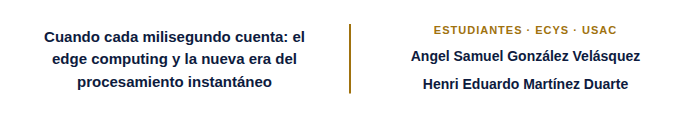
\includegraphics[width=1\linewidth]{labels/pareja23} \end{center}

\begin {multicols}{2}

\textbf{Palabras clave}\\
eficiencia operativa, transformación tecnológica, procesamiento local, digitalización, industria 4.0

\section{Introducción}\label{introducciuxf3n-2}

La velocidad del procesamiento ha dejado de ser un lujo tecnológico para convertirse en una necesidad. Durante años, el modelo dominante fue claro: enviar y procesar los datos en grandes centros de datos y de ahí devolver la respuesta. Pero al crecer la cantidad de información y las expectativas de inmediatez, ese recorrido empieza a resultar muy largo.

Es aquí donde emerge una nueva arquitectura: llevar el procesamiento al borde, justo donde los datos nacen. La inteligencia ya no se concentra en infraestructuras remotas; más bien es distribuida estratégicamente para ofrecer respuestas en tiempo real, reducir la latencia y optimizar recursos. Pasar de la nube al ``borde'' es un cambio de paradigma que está transformando industrias y marcando el inicio de la era del procesamiento instantáneo.

\section{Artículo}\label{artuxedculo-1}

El edge computing sitúa el procesamiento, almacenamiento y los servicios de red lo más cerca posible de donde se generan los datos. A diferencia de la nube tradicional, esta tecnología permite que el análisis ocurra de manera local, reduciendo la latencia, los tiempos de espera y la constante dependencia de una conexión estable a internet. Además, se fortalece la ciberseguridad, pues al procesar información sensible in situ, se minimiza la exposición de datos durante su transporte.

En el sector industrial, el mantenimiento predictivo ha transformado la fabricación y su calidad. Con ayuda de sensores, se puede detectar el desgaste de componentes en tiempo real, reduciendo significativamente el tiempo de mantenimiento. En la industria alimentaria, las cámaras de visión artificial procesan datos volumétricos localmente para ajustar la producción ante cambios de humedad o temperatura, estabilizando la calidad y reduciendo los costes por desperdicio de producto.

Sectores como el transporte inteligente dependen de esta arquitectura para gestionar el tráfico en tiempo real y evitar colisiones. Los vehículos autónomos requieren análisis de datos en milisegundos para navegar con seguridad, algo que solo el procesamiento en el borde permite. En el sector salud, el monitoreo constante de pacientes con dispositivos médicos locales ofrece respuestas rápidas y seguras sin los retrasos del procesamiento remoto, algo fundamental para situaciones de emergencia médica inmediata.

\begin{center}
\includegraphics[width=0.8\linewidth]{articulos_seleccionados/imagenes_articulos_seleccionados/A_pareja23/p1} \end{center}

\emph{Figura 1: Sectores críticos que demandan eficiencia y rapidez. Fuente: Elaboración propia.}

El verdadero éxito actual reside en adoptar un ecosistema híbrido donde el borde y la nube trabajan juntos. Mientras el borde gestiona decisiones urgentes y datos pesados localmente, la nube provee almacenamiento masivo y un análisis de todos estos datos a largo plazo. Esta combinación permite que las cargas de trabajo se desplieguen de forma óptima según la necesidad de inmediatez o de potencia computacional. Es la estrategia ideal para maximizar la escalabilidad y la eficiencia operativa en la industria 4.0.

\begin{center}
\includegraphics[width=0.8\linewidth]{articulos_seleccionados/imagenes_articulos_seleccionados/A_pareja23/p2} \end{center}

\emph{Figura 2: Modelo ``Edge Computing'' con participación de la nube. Fuente: IoT Application Expert.}

\section{Conclusiones}\label{conclusiones}

El paso de la nube al borde es un cambio que no solo reduce la latencia, sino que también mejora la seguridad, optimiza recursos y permite realizar decisiones críticas en tiempo real. Esto dejó de representar solo una ventaja para convertirse en un requisito necesario para competir.

Con el borde no se pretende sustituir a la nube: el borde resuelve lo urgente y la nube se encarga de consolidar, almacenar y analizar a gran escala. La sinergia entre el borde y la nube es lo que impulsa la transformación digital y la consolida como un pilar fundamental para el avance tecnológico actual.

\section{Bibliografía}\label{bibliografuxeda-2}

\begin{itemize}
\item
  Jessup University. ``Edge Computing vs.~Cloud Computing: Key Differences in 2024.'' Enero, 2024. \url{https://jessup.edu/blog/engineering-technology/edge-computing-vs-cloud-computing/}
\item
  Equipo SAAVY. ``Edge Computing En La Industria: Definición y Casos de Éxito.'' SAVVY DATA SYSTEMS, Julio, 2025.
\item
  Latorre, Lucia, et al.~``Reporte de Tecnología: Edge Computing.'' Banco Interamericano de Desarrollo (BID), 2024.
\end{itemize}

\end {multicols}

\medskip

\suppresschapterfalse

\articletitlecommand
\vspace*{-23mm}
\phantomsection
\label{pareja12}
\addcontentsline{toc}{chapter}{}

\chapter{Machine learning en producción: cuando los algoritmos deciden por nosotros}\label{pareja12}

\null\vspace*{-20mm}

\begin{center}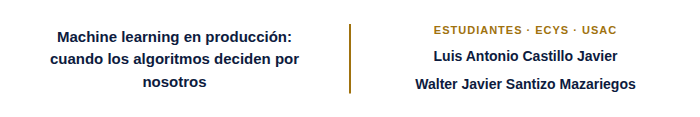
\includegraphics[width=1\linewidth]{labels/pareja12} \end{center}

\begin {multicols}{2}

\textbf{Palabras clave}\\
aprendizaje automático, productos digitales, personalización, sesgo algorítmico, experiencia de usuario

\section{Introducción}\label{introducciuxf3n-3}

Pensemos en una mañana cualquiera: abrimos Spotify y la primera canción que suena es exactamente lo que necesitábamos sin saberlo; revisamos el correo y los mensajes importantes ya están separados del resto; pagamos con tarjeta y, en milisegundos, un sistema decidió que esa transacción es legítima. Ninguna de esas cosas ocurren por accidente.

Lo llamativo de todo esto es que hace menos de una década, estas capacidades eran territorio casi exclusivo de grandes laboratorios de investigación. Hoy están en el teléfono de cualquier persona. El machine learning bajó de los papers académicos a las apps de uso diario, y ese salto no fue solo técnico: fue también un salto de responsabilidad.

\section{Artículo}\label{artuxedculo-2}

\textbf{Del desarrollo a la implementación}

Construir un producto que implemente técnicas o algoritmos de machine learning no es lo que normalmente pensamos. El proceso empieza mucho antes de la fase de análisis: hay que entender el problema que se quiere resolver y qué información o estudios previos existen para abordarlo. Un conjunto de datos se convierte en información sin sentido si no se cuenta con el análisis correcto bajo el contexto adecuado. Un modelo supervisado necesita ejemplos etiquetados de calidad; uno no supervisado puede encontrar estructuras sin etiquetas, pero esa estructura hay que interpretarla.

En cuanto al modelo entrenado, la prueba de fuego surge cuando llega a producción: es ahí donde verdaderamente surgen los fenómenos no anticipados, los sesgos se confirman y los datos del entrenamiento parecieran no tener relación con los del ``mundo real''. La latencia, que en sistemas de recomendación o detección de fraude puede marcar la diferencia entre una experiencia fluida y una que el usuario abandona.

\textbf{Del dato al producto}

Los sistemas de recomendación son quizás el caso más visible. Plataformas como Netflix o YouTube usan variantes de filtrado colaborativo y modelos de factorización matricial para estimar la probabilidad de que un usuario consuma cierto contenido. El resultado es una experiencia que se siente personalizada, aunque en realidad es probabilística.

El machine learning opera también en ciberseguridad: los sistemas de detección de fraude bancario trabajan con modelos de clasificación en tiempo real sobre millones de registros ---monto, ubicación, dispositivo, hora--- permitiendo detectar un patrón de gasto histórico que se compara con la transacción sospechosa. Lo mismo ocurre en salud digital, donde modelos de series de tiempo analizan señales de sensores para detectar síntomas antes de que el usuario los note.

\textbf{Sesgos, explicabilidad y lo que el usuario merece saber}

Un 95\% de precisión suena bien hasta que te preguntas quiénes componen el 5\% restante. Varios estudios han documentado casos donde modelos de reconocimiento facial o de evaluación crediticia cometen errores de forma desproporcionada en ciertos grupos demográficos, no por diseño malicioso, sino porque los datos de entrenamiento ya contenían esos desequilibrios. Este fenómeno, conocido como sesgo algorítmico, es uno de los problemas más estudiados en el campo actualmente.

A esto se suma el problema de la explicabilidad. Los modelos más potentes operan como cajas negras: producen salidas precisas pero difíciles de justificar. Herramientas como SHAP o LIME permiten aproximar explicaciones locales de las predicciones, pero son eso: aproximaciones.

\begin{center}
\includegraphics[width=0.8\linewidth]{articulos_seleccionados/imagenes_articulos_seleccionados/A_pareja12/p1} \end{center}

\emph{Figura 1: SHapley Additive exPlanation. Fuente: Shap Organization.}

\section{Conclusiones}\label{conclusiones-1}

El machine learning ya no es tecnología del futuro: está en el núcleo de los productos digitales que usamos a diario. Su poder real no está en los algoritmos en sí, sino en la combinación de buenos datos, decisiones de diseño conscientes y equipos dispuestos a hacerse responsables de lo que construyen. Un modelo que aprende rápido pero que nadie puede explicar, corregir o cuestionar, es un riesgo disfrazado de eficiencia. La diferencia entre un buen producto y uno dañino no siempre está en la precisión del modelo, sino en cómo el equipo responde cuando ese modelo se equivoca.

\section{Bibliografía}\label{bibliografuxeda-3}

\begin{itemize}
\item
  ``Large-Scale Machine Learning Systems in Real-World Industrial Settings.'' 2020. \emph{Information and Software Technology}. ScienceDirect.
\item
  ``Fairness Issues, Current Approaches, and Challenges in Machine Learning Models.'' 2023. \emph{International Journal of Machine Learning and Cybernetics}. Springer Nature.
\item
  ``Best Practices for Real-World ML Deployment.'' TechTarget. 2026.
\item
  ``ML Health: Fitness Tracking for Production Models.'' 2019. arXiv Preprint.
\item
  ``MLOps Challenges.'' ScienceDirect. 2026.
\end{itemize}

\end {multicols}

\medskip

\suppresschapterfalse

\articletitlecommand
\vspace*{-23mm}
\phantomsection
\label{pareja64}
\addcontentsline{toc}{chapter}{}

\chapter{El hash como huella digital matemática que blinda el blockchain}\label{pareja64}

\null\vspace*{-20mm}

\begin{center}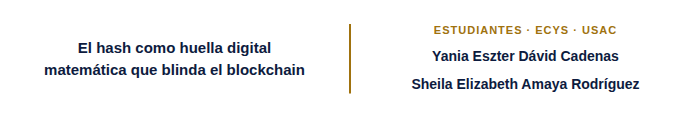
\includegraphics[width=1\linewidth]{labels/pareja64} \end{center}

\textbf{Palabras clave:} blockchain, hash, inmutabilidad, criptografía, seguridad digital.

\begin {multicols}{2}

\section{Introducción}\label{introducciuxf3n-4}

¿Es posible confiar ciegamente en un sistema digital donde cualquier dato podría ser alterado sin dejar rastro? En la arquitectura informática convencional, la centralización de los servidores crea puntos únicos de falla que vulneran la integridad de nuestra información más sensible. Esta fragilidad estructural nos obliga a buscar mecanismos donde la seguridad no dependa de la buena voluntad humana, sino de la robustez del código.

Aquí es donde la criptografía toma el control mediante una red distribuida que se encarga de vigilar cada bit de datos. Al utilizar algoritmos de hash, la confianza se transforma en una propiedad técnica inalterable que blinda la verdad dentro de una cadena de bloques. Comprender este engranaje matemático nos permite visualizar un entorno digital donde la transparencia y la honestidad son, por primera vez, garantías inviolables por diseño.

\section{Desarrollo}\label{desarrollo-1}

El mayor riesgo en una comunicación digital no es solo que el mensaje sea interceptado, sino que este sea suplantado o modificado sin que el receptor lo note. Se define la autenticidad como la garantía de que un mensaje proviene realmente del emisor legítimo y no ha sido alterado en el camino (Simmons 1985). Esta premisa es la base de blockchain: pasar de una confianza basada en la buena voluntad a una blindada por protocolos matemáticos que eliminan cualquier margen de engaño.

\begin{center}
\includegraphics[width=0.8\linewidth]{articulos_seleccionados/imagenes_articulos_seleccionados/A_pareja64/p1} \end{center}

\emph{Figura 1. Esquema general de un sistema de autenticación. Fuente: Simmons (1985).}

Para materializar esta visión de autenticidad, se utiliza el algoritmo SHA-256 como el eje fundamental de seguridad. Este mecanismo toma cualquier volumen de datos y lo traduce en una cadena de 64 caracteres que actúa como una huella digital única. Lo interesante es el determinístico técnico: cualquier cambio mínimo en el texto original genera un hash completamente distinto. Esta propiedad permite que cada nodo de la red verifique la integridad del bloque de forma instantánea y autónoma, asegurando que la información sea realmente inmutable y transparente para todos los participantes.

\begin{center}
\includegraphics[width=0.8\linewidth]{articulos_seleccionados/imagenes_articulos_seleccionados/A_pareja64/p2} \end{center}

\emph{Figura 2. Conversión de bloques mediante hash SHA-256. Fuente: Díaz Gutiérrez y Cueva Lovelle (2018).}

La verdadera innovación ocurre al vincular estos hashes en una secuencia lógica. Cada bloque nuevo arrastra el PreviousHash del anterior. Como propuso Nakamoto (2008), este diseño crea un historial cronológico inalterable que no puede ser modificado sin rehacer todo el trabajo computacional de la red. Si se intentara alterar un registro pasado, se rompería la coherencia de toda la cadena subsiguiente, invalidando el esfuerzo de los nodos. Es un sistema donde la honestidad es la única ruta técnica posible para que un bloque sea aceptado por el consenso distribuido.

\begin{center}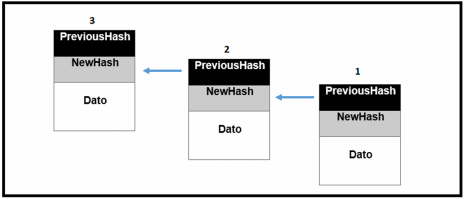
\includegraphics[width=0.8\linewidth]{articulos_seleccionados/imagenes_articulos_seleccionados/A_pareja64/p3} \end{center}

\emph{Figura 3. Modelo de comunicación de cadenas de bloques por medio de hash. Fuente: Díaz Gutiérrez y Cueva Lovelle (2018).}

Para que este enlazamiento sea verdaderamente resistente a ataques, el proceso requiere del Nonce, un número aleatorio que funciona como la pieza final del rompecabezas de seguridad. Este componente asegura que generar un bloque sea costoso en procesamiento, pero sencillo de verificar para el resto de los participantes.

Al integrar el índice, el hash anterior y el Nonce, se logra un esquema de control que protege la información de posibles ataques, garantizando la integridad de los datos durante toda su transmisión. Entender cómo esta tecnología blinda la verdad digital permite visualizar un futuro donde la integridad de los datos es, por fin, una certeza absoluta.

\section{Conclusión}\label{conclusiuxf3n-2}

El éxito del Blockchain no radica en la tecnología por sí misma, sino en el cómo se traslada la confianza. Al combinar la inmutabilidad del SHA-256 con los pilares de la autenticidad que Simmons planteó, logramos que la integridad de los datos deje de ser una simple buena intención para volverse una certeza técnica que nadie puede cuestionar. Este modelo no se limita a frenar suplantaciones; levanta un muro de transparencia real frente a cualquier control centralizado que pretenda manipular la verdad digital. Dominar estos engranajes nos permite proyectar un entorno donde cada transacción electrónica sea segura por su propia naturaleza matemática. Estos protocolos distribuidos son el escudo definitivo contra las grietas de los servidores tradicionales, blindando la información mediante un consenso de red que garantiza un sellado criptográfico permanente y transparente para todos.

\section{Bibliografía}\label{bibliografuxeda-4}

\begin{itemize}
\item
  Díaz Gutiérrez, Yesid, y Juan Manuel Cueva Lovelle. ``Análisis de la función Hash Criptográfica en cadenas de bloques y su impacto en la seguridad de transacciones de datos.'' \emph{Redes de Ingeniería} 9, n.º 2 (2018): 82-87. \url{https://doi.org/10.14483/2248762X.14383}.
\item
  Nakamoto, Satoshi. \emph{Bitcoin: A Peer-to-Peer Electronic Cash System}. Bitcoin.org, 2008. \url{https://bitcoin.org/bitcoin.pdf}.
\item
  Simmons, Gustavus J. ``Authentication Theory/Coding Theory.'' En \emph{Advances in Cryptology (CRYPTO '84)}, editado por G. Blakley y D. Chaum, 411-431. Berlín: Springer-Verlag, 1985. \url{https://doi.org/10.1007/3-540-39568-7_32}.
\end{itemize}

\end {multicols}

\medskip

\suppresschapterfalse
\clearpage
\suppressbackgroundtrue

\includepdf[pages=1,fitpaper=true]{articulos_seleccionados/images/seccion2.pdf}
\suppressbackgroundfalse

\clearpage
\let\origclearpage\clearpage
\let\origcleardoublepage\cleardoublepage
\let\clearpage\relax
\let\cleardoublepage\relax
\articletitleafterpdfsection
\phantomsection
\label{entrevista02_JuliOron}
\addcontentsline{toc}{chapter}{}

\chapter{El futuro del desarrollo de software con inteligencia artificial}\label{entrevista02_JuliOron}

\let\clearpage\origclearpage
\let\cleardoublepage\origcleardoublepage

\null\vspace*{-20mm}

\begin{center}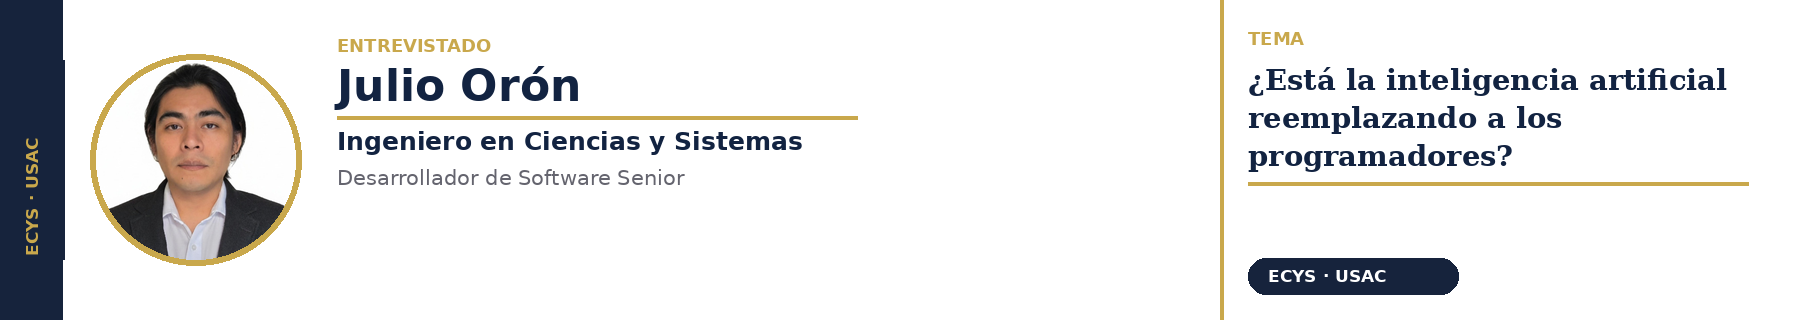
\includegraphics[width=1\linewidth]{etiquetas_ingenieros/ing2} \end{center}

\begin {multicols}{2}

\textbf{\emph{YouTube:}} \url{https://youtu.be/5lokN1-N8rgc}

\section{Entrevista}\label{entrevista-1}

\textbf{¿Quién es Julio Orón?}

Mi nombre es Julio Orón y me desempeño como desarrollador de software. Actualmente trabajo en una empresa de telemedicina, donde ocupo el rol de desarrollador de software senior. Dentro de la organización, además de mis funciones técnicas, también participo en procesos de liderazgo y coordinación con el equipo, apoyando en la toma de decisiones y en la ejecución de proyectos tecnológicos.

Mi experiencia se ha enfocado en el desarrollo de software y en la adaptación a nuevas tecnologías, especialmente en el contexto actual donde la inteligencia artificial está transformando la industria. A lo largo de mi carrera he buscado mantenerme actualizado, entendiendo no solo las herramientas, sino también el impacto que estas tienen en el entorno laboral.

\textbf{¿Cómo fue su camino hasta llegar a su posición actual en el área tecnológica?}

Mi camino en la tecnología comenzó en un contexto bastante distinto al actual. En el lugar donde vivía, el acceso a computadoras era limitado; únicamente existía un café internet, y todo lo relacionado con la tecnología era completamente nuevo. Mis primeros acercamientos fueron a través de cursos básicos, como Excel, lo cual despertó mi interés por este campo.

Cuando decidí estudiar la carrera, realmente no tenía claridad sobre lo que implicaba ser desarrollador de software. Sin embargo, conforme avancé en mi formación, fui comprendiendo el alcance de la disciplina. Inicié en el año 2010 como programador junior y, con el tiempo, fui adquiriendo experiencia, creciendo profesionalmente y asumiendo mayores responsabilidades hasta convertirme en desarrollador senior.

Este proceso ha sido continuo, caracterizado por el aprendizaje constante y la adaptación a cambios tecnológicos. Uno de los aspectos que más me ha motivado es la flexibilidad que ofrece el área, especialmente el trabajo remoto y las oportunidades de crecimiento profesional.

\textbf{¿Qué relación tiene su trabajo con la inteligencia artificial en la actualidad?}

La inteligencia artificial está teniendo un impacto significativo en el desarrollo de software, especialmente en la generación de código. Actualmente, muchas de las tareas que antes realizaban los programadores de forma manual están siendo automatizadas.

Esto ha generado un cambio importante en el rol del desarrollador. Más que desaparecer, la función está evolucionando hacia la gestión de herramientas de inteligencia artificial. Además, ha surgido una nueva área enfocada en el entrenamiento de modelos, donde la experiencia de los desarrolladores es fundamental.

Si bien existe la percepción de que la IA puede reemplazar a los programadores, en realidad lo que está ocurriendo es una transformación del perfil profesional, donde se requiere mayor capacidad de análisis, supervisión y toma de decisiones.

\textbf{¿Cómo ha impactado la inteligencia artificial en su forma de trabajar?}

El impacto ha sido considerable. Actualmente utilizo inteligencia artificial para la generación de código, lo que ha reducido significativamente el tiempo de desarrollo. Antes, el trabajo implicaba escribir grandes cantidades de código manualmente, lo cual generaba presión por los tiempos de entrega y, en algunos casos, afectaba la salud física debido al esfuerzo constante.

Con la IA, este proceso se ha optimizado. Ahora es posible generar soluciones en menos tiempo, con mejor calidad y mayor nivel de seguridad. Esto no implica que el desarrollador sea reemplazado, sino que su enfoque cambia hacia la validación, integración y optimización del trabajo generado por la herramienta.

\textbf{¿Confía en el código generado por inteligencia artificial?}

Sí, existe un alto nivel de confianza en el código generado por la inteligencia artificial. Sin embargo, no se trata de una confianza absoluta sin validación. Dado que la IA puede generar grandes volúmenes de código en cuestión de segundos, resulta poco práctico revisar cada línea.

En su lugar, el enfoque actual consiste en evaluar patrones, verificar la funcionalidad, y asegurar que el sistema cumpla con criterios de optimización y seguridad. Uno de los principales retos es el manejo del contexto, ya que la IA puede generar soluciones correctas de forma aislada, pero puede presentar dificultades al integrarlas en sistemas más complejos.

\textbf{¿Considera que la inteligencia artificial ya puede desarrollar sistemas completos?}

La inteligencia artificial ya tiene la capacidad de desarrollar sistemas completos, aunque esto depende del nivel de complejidad. En sistemas simples, es posible generar soluciones funcionales si se proporciona la guía adecuada.

En mi experiencia personal, he logrado desarrollar sistemas completos utilizando inteligencia artificial, incluso trabajando con tecnologías que no conocía previamente. Sin embargo, en proyectos más complejos, sigue siendo necesaria la intervención humana para estructurar, integrar y validar las soluciones.

\textbf{¿Qué opinión tiene sobre los sesgos en la inteligencia artificial?}

Los sesgos en la inteligencia artificial no son un fenómeno aislado, sino un reflejo de los sesgos presentes en la sociedad. La IA se entrena con datos generados por humanos, por lo que inevitablemente incorpora ciertos patrones y prejuicios.

Desde mi perspectiva, esto no representa una preocupación mayor, ya que los sistemas tienden a corregirse con el tiempo, especialmente debido a factores económicos y sociales que incentivan su mejora. En este sentido, la inteligencia artificial puede entenderse como una extensión del comportamiento humano.

\textbf{¿Quién considera que es responsable cuando un sistema con IA comete un error?}

La responsabilidad recae en el usuario. La inteligencia artificial es una herramienta que facilita el procesamiento de información, pero la toma de decisiones sigue siendo responsabilidad del ser humano.

El uso incorrecto de la información generada por IA puede generar errores o problemas, pero estos no son atribuibles a la herramienta en sí, sino a la forma en que se utiliza. Por ello, es fundamental que los profesionales actúen con criterio y responsabilidad al emplear estas tecnologías.

\textbf{¿Qué tecnologías emergentes relacionadas con IA le generan mayor interés?}

Más que una tecnología específica, lo que resulta más interesante es el desarrollo de la inteligencia artificial en general. Sin embargo, uno de los avances más prometedores es la posible integración con la computación cuántica, lo cual podría acelerar significativamente su evolución.

Asimismo, la combinación de inteligencia artificial con robótica podría transformar profundamente la producción y la organización social, abriendo nuevas posibilidades en distintos sectores.

\textbf{¿Qué consejo daría a los estudiantes de ingeniería en sistemas?}

El principal consejo es no depender completamente de la inteligencia artificial. Si bien es una herramienta poderosa, es fundamental seguir desarrollando habilidades cognitivas como el pensamiento crítico, el análisis y la creatividad.

Así como en el pasado la tecnología reemplazó el esfuerzo físico, actualmente está comenzando a reemplazar parte del esfuerzo cognitivo. Por ello, es importante utilizar la IA como complemento y no como sustituto total de nuestras capacidades.

\textbf{Mensaje final de Julio Orón}

La inteligencia artificial representa una oportunidad para mejorar la productividad y la calidad de vida. Sin embargo, su uso debe ser consciente y estratégico. El verdadero valor no está en la herramienta, sino en la capacidad del profesional para adaptarse, aprender y evolucionar junto con la tecnología.

\end {multicols}

\medskip

\HRule

\medskip

\suppresschapterfalse

\articletitlecommand
\phantomsection
\label{pareja26}
\addcontentsline{toc}{chapter}{}

\chapter{De Desarrollador a Supervisor: programar con IA no es cheat, es skill}\label{pareja26}

\null\vspace*{-20mm}

\begin{center}
\includegraphics[width=1\linewidth]{labels/pareja26} \end{center}

\begin {multicols}{2}

\textbf{Palabras clave}\\
inteligencia artificial, ingeniería de software, paradigmas de programación, competencias tecnológicas, abstracción

\section{Introducción}\label{introducciuxf3n-5}

Actualmente, la programación ya no es ni parecida a lo que nos enseñaron cuando empezamos a programar, sudando frente a la pantalla para escribir un simple ``Hello World'' o pasando horas de madrugada buscando un punto y coma perdido. Ahorita ya hay herramientas que nos dan el código completo en cuestión de segundos, y eso ha dado muchísimo de qué hablar en nuestro entorno de la facultad.

Hay gente purista que dice que es una trampa, que ya nadie aprende de verdad, y otros que dicen que, al contrario, que es parte de evolucionar para no quedarnos estancados con prácticas viejas. En las universidades y en el trabajo el debate está vivo: ¿usar estas cosas nos está poniendo haraganes o nos está preparando para lo que viene en el mercado laboral?

\section{Artículo}\label{artuxedculo-3}

En el mundo del desarrollo, decirle ``cheat'' a algo significa que estás haciendo trampa para saltarte el trabajo duro. Muchos desarrolladores todavía creen que, si no te quiebras la cabeza escribiendo todo desde cero, no eres un ingeniero de verdad. Sienten que usar la inteligencia artificial para armar la base de un proyecto es quitarle todo el mérito y la lógica a la programación.

Pensar que apoyarse en la inteligencia artificial es hacer trampa es ignorar la historia de nuestra propia carrera. Es, sencillamente, el siguiente nivel de abstracción tecnológica que nos permite avanzar mucho más rápido. Este cambio de paradigma transforma por completo nuestro rol tradicional: pasamos de ser simples digitadores a verdaderos arquitectos del código. La generación de código base pasa de ser manual a automatizada; el rol del ingeniero evoluciona de codificador a supervisor y auditor de lógica; y el enfoque del tiempo se desplaza de la mecánica de la escritura al diseño, la seguridad y la escalabilidad.

Aquí es donde ocurre nuestro cambio de rol: pasamos de ser los que solo tiran líneas, a ser los supervisores de la obra. Analógicamente, toca revisar qué está haciendo el asistente, cómo lo está integrando y si realmente cumple con los requisitos solicitados. También formular la instrucción correcta requiere saber exactamente qué formas de datos necesitas usar.

De hecho, los entornos de desarrollo integrados llevan años dándonos una mano. Un ejemplo clarísimo de esto es lo que se muestra en la Figura 1, donde el asistente detecta un error de tipeo en una variable durante un pull request y sugiere la corrección exacta al instante. Que ahora una inteligencia artificial nos pueda generar un bloque entero de código es solo el siguiente paso lógico en esta cadena. No es trampa, es la tecnología optimizando nuestro tiempo de trabajo.

\begin{center}
\includegraphics[width=0.8\linewidth]{articulos_seleccionados/imagenes_articulos_seleccionados/A_pareja26/p1} \end{center}

\emph{Figura 1: Ejemplo de revisión automática de código en un pull request con asistente de IA. Fuente: GitHub Copilot en GitHub Documentation (2024).}

\section{Conclusión}\label{conclusiuxf3n-3}

La integración de la inteligencia artificial en el desarrollo de software no representa una amenaza para la labor del ingeniero, sino una transformación que eleva el nivel de competencias requeridas. Sostener que el uso de estas herramientas constituye una práctica deshonesta implica desconocer la evolución histórica de la abstracción tecnológica y las demandas actuales del mercado laboral.

Sin una comprensión sólida de los fundamentos lógicos y estructurales de la programación, el uso indiscriminado de estas herramientas puede derivar en soluciones deficientes que comprometan la estabilidad de los sistemas en entornos de producción. En consecuencia, dominar el uso estratégico de la inteligencia artificial como herramienta de apoyo constituye una competencia técnica fundamental para el ingeniero del siglo XXI.

\section{Bibliografía}\label{bibliografuxeda-5}

\begin{itemize}
\item
  GitHub, Inc.~``Using Copilot for Code Review.'' \emph{GitHub Documentation}. 2024. \url{https://docs.github.com/en/copilot/using-github-copilot/code-review/using-copilot-code-review}.
\item
  O'Reilly, Tim. \emph{La inteligencia artificial en el desarrollo de software}. Madrid: Ediciones Técnicas, 2023.
\item
  Parnin, Chris, y Sarah D'Angelo. ``Generación de código asistida por IA: Retos y oportunidades.'' \emph{Revista de Ingeniería de Software} 15, no. 2 (2024): 45--60.
\item
  Treude, Christoph. \emph{El nuevo paradigma del programador: De codificador a supervisor}. Chicago: Tech Press, 2023.
\end{itemize}

\end {multicols}

\medskip

\suppresschapterfalse

\articletitlecommand
\vspace*{-23mm}
\phantomsection
\label{pareja67}
\addcontentsline{toc}{chapter}{}

\chapter{Orquestando el futuro: el ingeniero en entornos automatizados}\label{pareja67}

\null\vspace*{-20mm}

\begin{center}
\includegraphics[width=1\linewidth]{labels/pareja67} \end{center}

\textbf{Palabras clave:} automatización, CI/CD, evolución del ingeniero, orquestación, DevSecOps, infraestructura como código.

\begin {multicols}{2}

\section{Introducción}\label{introducciuxf3n-6}

La integración de la IA y los entornos automatizados ha desplazado el enfoque desde el código manual hacia la orquestación sistémica. Esta evolución marca el fin de las tareas repetitivas, permitiendo que el ingeniero se centre en la gestión estratégica de alto nivel. Históricamente, el rol era puramente operativo, pero hoy exige una visión integral y profunda de los ecosistemas digitales modernos.

El objetivo de este análisis es explorar la metamorfosis del ingeniero dentro de los flujos de trabajo de CI/CD y DevOps. Se busca comprender cómo el profesional transita de ser un simple ejecutor a un arquitecto de resiliencia que garantiza la gobernanza ética de los sistemas. Esta transición es vital para mantener la relevancia ante el procesamiento masivo de datos en la industria actual.

\section{Desarrollo}\label{desarrollo-2}

Históricamente, el ingeniero de sistemas invertía la mayor parte de su tiempo en tareas operativas y repetitivas. Configurar servidores de forma manual y hacer pruebas paso a paso limitaban enormemente la innovación. Hoy ese enfoque representa una desventaja competitiva real frente a entornos automatizados que procesan, prueban y despliegan código sin intervención humana. El cambio más significativo en este paradigma es el paso de ``constructor'' a ``orquestador'': ya no se trata de fabricar el ladrillo, sino de diseñar la fábrica completa que lo produce.

\end {multicols}

\begin{longtable}[]{@{}
  >{\raggedright\arraybackslash}p{(\linewidth - 4\tabcolsep) * \real{0.3333}}
  >{\raggedright\arraybackslash}p{(\linewidth - 4\tabcolsep) * \real{0.3333}}
  >{\raggedright\arraybackslash}p{(\linewidth - 4\tabcolsep) * \real{0.3333}}@{}}
\toprule\noalign{}
\begin{minipage}[b]{\linewidth}\raggedright
Aspecto
\end{minipage} & \begin{minipage}[b]{\linewidth}\raggedright
Ingeniero Tradicional
\end{minipage} & \begin{minipage}[b]{\linewidth}\raggedright
Ingeniero Moderno
\end{minipage} \\
\midrule\noalign{}
\endhead
\bottomrule\noalign{}
\endlastfoot
Rol principal & Ejecutor operativo & Orquestador de sistemas \\
Gestión de entornos & Manual & Infraestructura como Código \\
Relación con errores & Reactiva & Preventiva y automatizada \\
Seguridad & Al final del proyecto & Integrada desde el inicio \\
Valor diferenciador & Velocidad de código & Pensamiento crítico y visión de negocio \\
\end{longtable}

\emph{Figura 7.1. Comparación ingeniero tradicional vs ingeniero moderno. Fuente: Elaboración propia.}

\begin {multicols}{2}

La Infraestructura como Código (IaC) y los pipelines de CI/CD son el núcleo de esta transformación. Herramientas como Terraform, Kubernetes y GitHub Copilot han redefinido lo que significa ser competente en la industria. Dominar estas herramientas es hoy parte esencial del perfil profesional, junto con seguridad, observabilidad y estrategias multi-nube. La habilidad diferenciadora ya no es escribir código rápido, sino saber orquestar, automatizar y validar cada parte del flujo de entrega.

La automatización no solo optimiza tiempos, sino que también redefine la toma de decisiones dentro del ciclo de vida del software. Las métricas de OpenTelemetry permiten recopilar datos en tiempo real sobre el rendimiento de aplicaciones e infraestructura, habilitando a los equipos DevOps para utilizarlas como sistema de alerta temprana ante posibles fallos. Esta capacidad analítica transforma al ingeniero en un estratega que interpreta información crítica para anticipar fallos antes de que impacten al usuario final. La observabilidad se convierte así en un pilar tan importante como el código mismo.

Asimismo, la adopción de arquitecturas basadas en contenedores y microservicios ha incrementado la complejidad estructural de los sistemas. Esta fragmentación exige una visión sistémica para garantizar interoperabilidad, escalabilidad y tolerancia a fallos. En este contexto, herramientas como Kubernetes no solo automatizan despliegues, sino que permiten gestionar ecosistemas distribuidos con alta resiliencia. El ingeniero moderno debe comprender no solo cómo funciona cada componente, sino cómo interactúan entre sí dentro del entorno productivo.

Por otra parte, la integración de inteligencia artificial en los pipelines de CI/CD está acelerando la detección de vulnerabilidades y la generación de pruebas automatizadas. Según el Global DevSecOps Report 2024 de GitLab, la adopción de automatización avanzada y herramientas asistidas por IA está directamente vinculada con ciclos de entrega más rápidos y menor exposición a riesgos de seguridad. Esto no elimina la responsabilidad humana, sino que la eleva hacia la supervisión ética y la validación estratégica de resultados.

\begin{center}
\includegraphics[width=0.8\linewidth]{articulos_seleccionados/imagenes_articulos_seleccionados/A_pareja67/p1} \end{center}

\emph{Figura 7.2. Flujo DevSecOps y enfoque ``shift left''. Fuente: Snyk.}

Bajo la filosofía DevSecOps, la seguridad deja de ser un paso final para convertirse en una responsabilidad integrada desde el primer commit. Según el Reporte Global DevSecOps 2024 de GitLab, elaborado con más de 5,000 profesionales en 39 países, la seguridad se consolidó como la principal prioridad de inversión en TI. Este es el cambio cultural más profundo de la industria: el ingeniero moderno no solo programa, sino que orquesta sistemas resilientes, seguros y capaces de adaptarse a las necesidades del negocio.

\section{Conclusiones}\label{conclusiones-2}

La transformación del ingeniero de sistemas representa una evolución estructural impulsada por la automatización, la inteligencia artificial y la integración de la seguridad desde las primeras fases del desarrollo. Los datos del Reporte Global DevSecOps 2024 de GitLab confirman que la seguridad y la automatización son los ejes centrales de la estrategia tecnológica empresarial. El profesional que comprenda esto y se adapte tendrá una ventaja competitiva real; quien no lo haga quedará rezagado frente a entornos que evolucionan constantemente. La clave no está en competir contra las herramientas de IA, sino en aprender a dirigirlas con juicio crítico y responsabilidad ética. Se recomienda que las instituciones educativas actualicen sus programas para incluir competencias como IaC, DevSecOps y trabajo colaborativo con IA.

\section{Bibliografía}\label{bibliografuxeda-6}

\begin{itemize}
\item
  GitLab Inc.~\emph{The Global DevSecOps Report 2024}. San Francisco: GitLab, 2024. \url{https://about.gitlab.com/developer-survey/}
\item
  KodeKloud. ``DevOps Skills 2025: Key Skills, Trends \& Training.'' \url{https://kodekloud.com/blog/devops-skills-2025}
\item
  IBM. ``OpenTelemetry Metrics: An Introduction.'' \url{https://www.ibm.com/think/topics/opentelemetry-metrics}
\item
  Snyk. ``What Is DevSecOps.'' \url{https://snyk.io/learn/devsecops}
\end{itemize}

\end {multicols}

\medskip

\suppresschapterfalse

\articletitlecommand
\vspace*{-23mm}
\phantomsection
\label{pareja6}
\addcontentsline{toc}{chapter}{}

\chapter{No te va a quitar el trabajo una IA, te lo va a quitar alguien que sabe usarla mejor que tú}\label{pareja6}

\null\vspace*{-20mm}

\begin{center}
\includegraphics[width=1\linewidth]{labels/pareja6} \end{center}

\begin {multicols}{2}

\textbf{Palabras clave}\\
inteligencia artificial, programación, adaptación, ventaja competitiva

\section{Introducción}\label{introducciuxf3n-7}

Hubo un momento en la historia reciente en que el internet era el enemigo. Las escuelas lo prohibían, las universidades solo aceptaban la biblioteca como fuente válida, y la desconfianza hacia esa nueva tecnología era la postura más común. Nadie quería adaptarse a algo tan desconocido y diferente a todo lo que existía antes. Hoy, quien no usa internet está desactualizado y perdiendo oportunidades en tiempo real.

Y la historia, con una precisión inquietante, está a punto de repetirse. Exactamente lo mismo está sucediendo ahora con la Inteligencia Artificial: se quiere prohibir, se le teme. Lo que antes se rechazaba por miedo, terminó siendo indispensable, y quienes no vean esto a tiempo con la IA, van a llegar tarde otra vez.

\section{Artículo}\label{artuxedculo-4}

\textbf{Las ventajas: lo que cambia cuando la usas bien}

En el mundo de la programación, la diferencia entre alguien que usa IA y alguien que no, se empieza a notar desde el primer proyecto. El desarrollador que la integra a su flujo de trabajo llega a resultados en menor tiempo, detecta y reduce errores antes de que se conviertan en un problema, optimiza su código sin tener que revisar documentación durante horas, y mejora la seguridad de sus aplicaciones con sugerencias que antes requerían experiencia de años.

Mientras un estudiante sin IA pasa dos horas buscando por qué su código no compila, otro con IA ya identificó el error, lo corrigió, entendió por qué ocurrió y ya está avanzando en el siguiente módulo. Esa diferencia, multiplicada por semanas, meses y proyectos, se convierte en experiencia, velocidad y ventaja competitiva real.

\textbf{Los desafíos: lo que pasa cuando te acomodas demasiado}

Pero aquí viene la parte que nadie quiere decir en voz alta: la IA también te puede volver cómodo, y esa comodidad tiene un precio. Según Nexus Integra, uno de los principales obstáculos es la escasez de perfiles con habilidades y experiencia en el tiempo requerido para la implementación, lo que refleja una falta de profesionales cualificados en la industria.

Cuando le pides a la IA que te resuelva cada problema sin intentar entenderlo primero, tu mente deja de ejercitarse. Dejas de desarrollar el criterio para identificar cuándo una solución es buena y cuándo es un desastre disfrazado de código limpio. Porque sí, la IA se equivoca. Genera código que compila pero que no hace lo que debería, sugiere soluciones que funcionan en teoría pero fallan en producción, y a veces simplemente inventa cosas con una confianza impresionante.

Como señala Paul Ford, ``¿El software que estoy haciendo para mí en mi teléfono es tan bueno como el código hecho a mano y a medida? No.~Pero es inmediato y barato\ldots{} podría fallar en la prueba de calidad de una empresa, pero cumpliría todos los plazos.''

Sin embargo, las empresas quieren personas que sepan usar la Inteligencia Artificial. Como se observa en la Ilustración 1, las empresas que utilizan IA tienen una probabilidad mayor de aumentar sus ingresos.

\begin{center}
\includegraphics[width=0.8\linewidth]{articulos_seleccionados/imagenes_articulos_seleccionados/A_pareja6/p1} \end{center}

\emph{Ilustración 1: Empresas Líderes en Inteligencia Artificial. Fuente: Iplytics.}

Los ingenieros que van a destacar en los próximos años no serán los que sepan más de memoria ni los que se nieguen a usar nuevas herramientas, sino aquellos que sepan combinar su conocimiento con el poder de la IA. Como concluye el Illinois Institute of Technology, el futuro de la programación no es una batalla entre humanos y máquinas, sino una colaboración. Al final, la IA no te va a quitar el trabajo. Te lo va a quitar alguien que colabore mejor con ella.

\section{Conclusión}\label{conclusiuxf3n-4}

La Inteligencia Artificial no es el fin de los programadores, es el inicio de una nueva forma de serlo. El miedo inicial va a ceder, la resistencia va a desaparecer, y lo que hoy se debate si usar o no, mañana va a ser un requisito básico en cualquier oferta de trabajo. La transformación ya comenzó, la pregunta es si vas a ser parte de los que la lideran o de los que la observan desde afuera. Para los estudiantes y futuros ingenieros el mensaje es claro: aprendan los fundamentos, desarrollen su criterio propio, y con esa base sólida integren la IA como su mejor herramienta. No la usen para evitar pensar, úsenla para pensar más lejos.

\section{Bibliografía}\label{bibliografuxeda-7}

\begin{itemize}
\item
  ADEN Business School. ``Inteligencia Artificial: Casos de Éxito Empresarial.'' Business Magazine. Consultado el 21 de marzo de 2026. \url{https://www.aden.org/business-magazine/inteligencia-artificial-casos-de-exito-empresarial/}.
\item
  Ford, Paul. ``La disrupción de la IA que estábamos esperando ha llegado.'' The New York Times, 19 de febrero de 2026.
\item
  Illinois Institute of Technology. ``Is AI a Coder's Friend or Foe?'' Consultado el 21 de marzo de 2026.
\item
  Nexus Integra. ``Ventajas y desventajas de la inteligencia artificial en empresas.'' 26 de julio de 2022.
\end{itemize}

\end {multicols}

\medskip

\suppresschapterfalse

\articletitlecommand
\vspace*{-23mm}
\phantomsection
\label{pareja29}
\addcontentsline{toc}{chapter}{}

\chapter{De la imaginación a la realidad: automatización del desarrollo con DevOps}\label{pareja29}

\null\vspace*{-20mm}

\begin{center}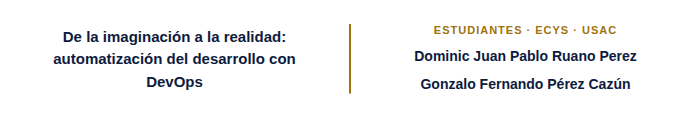
\includegraphics[width=1\linewidth]{labels/pareja29} \end{center}

\begin {multicols}{2}

\textbf{Palabras clave}\\
optimización, mejora, estabilidad, unión y desarrollo

\section{Introducción}\label{introducciuxf3n-8}

DevOps es una metodología que integra procesos en el desarrollo (Dev) y operaciones (Ops), con el objetivo de automatizar e integrar procesos en un ciclo de vida del software. Surge para eliminar la problemática de comunicación y coordinación entre equipos, evitando errores que causan la búsqueda de un responsable, si fue quien lo diseñó o del que lo desarrolló ---lo que se conoce como ``El Muro de la Confusión''.

Este enfoque permite a las organizaciones responder con mayor rapidez a los cambios del entorno y a las necesidades del usuario. De esta manera, se logra no solo acelerar el desarrollo, sino también garantizar entregas continuas con mayor calidad. En consecuencia, DevOps se convierte en un pilar fundamental en el desarrollo de software moderno.

\section{Artículo}\label{artuxedculo-5}

\textbf{Fases de DevOps}

DevOps es un conjunto de prácticas que abarcan todo el ciclo de vida del desarrollo de software. El proceso inicia con la fase de Plan, donde se definen los objetivos y requisitos del sistema. En Code se desarrolla el software, el cual en Build se integra automáticamente en un repositorio central. Siguiendo con el Test, se evalúa su correcto funcionamiento con pruebas automatizadas. En Release, se prepara el software para producción, y en Deploy se realiza su despliegue de forma rápida y consistente. Finalmente, en Operate y Monitor se supervisa y recopilan métricas para detectar fallos y mejorar continuamente el sistema, como se puede observar en la Figura 1.

\begin{center}
\includegraphics[width=0.8\linewidth]{articulos_seleccionados/imagenes_articulos_seleccionados/A_pareja29/p1} \end{center}

\emph{Figura 1: Diagrama del ciclo de vida del Software. Fuente: Elaboración propia, bajo las etapas definidas por IBM.}

\textbf{Automatización}

Amazon Web Services define DevOps como una combinación de prácticas culturales y herramientas que ``incrementan la capacidad de una organización para entregar aplicaciones y servicios a alta velocidad''. En el ciclo de vida del software, esto se presenta en la integración continua (CI) y el despliegue continuo (CD), que GitLab CI/CD define como ``parte de DevOps y combina las prácticas de integración continua y entrega continua.''

Todo inicia con el uso de sistemas de control de versiones como Git y técnicas de estructura como GitFlow, en el cual se almacenan y gestionan el código fuente. Cada cambio realizado activa automáticamente un pipeline de integración continua mediante herramientas de GitLab CI/CD. Posteriormente, el software puede empaquetarse en contenedores utilizando Docker, lo que garantiza que el entorno de ejecución sea consistente en cualquier servidor. Finalmente, el despliegue continuo permite publicar servicios en la nube como AWS.

\textbf{Beneficios: optimización, mejora, estabilidad}

DevOps aporta optimización al desarrollo de software porque automatiza procesos, mejora la comunicación entre equipos y reduce el tiempo de entrega. Esto permite trabajar de forma más eficiente y con menos fricciones entre desarrollo y operaciones (Almeida, Simões, and Lopes 2022).

Además, DevOps favorece la mejora continua y la estabilidad del software, ya que impulsa prácticas de aseguramiento de calidad, monitoreo y validación constante. Esto contribuye a reducir fallos, mejorar la calidad del sistema y ofrecer productos más confiables (Al Mohamad Saleh and Alzahrani 2023).

\section{Conclusiones}\label{conclusiones-3}

DevOps integra desarrollo y operaciones para automatizar procesos y mejorar la colaboración. Su aplicación optimiza el trabajo al reducir tiempos, tareas manuales y problemas de coordinación. También fortalece la calidad y la estabilidad del software mediante control, validación y mejora continua, permitiendo una entrega continua de software y facilitando la rápida adaptación a cambios del mercado y a nuevas necesidades del usuario. Gracias a la automatización de pruebas y despliegues, se disminuye significativamente el riesgo de errores en producción. En conjunto, DevOps se convierte en un enfoque clave para el desarrollo moderno de software.

\section{Bibliografía}\label{bibliografuxeda-8}

\begin{itemize}
\item
  Amazon Web Services. ``¿Qué es DevOps?'' Consultado el 20 de febrero de 2026. \url{https://aws.amazon.com/es/devops/what-is-devops/}
\item
  GitLab. ``¿Qué es CI/CD?'' Consultado el 24 de febrero de 2026. \url{https://about.gitlab.com/es/topics/ci-cd/}
\item
  Almeida, Fernando, Jorge Simões, and Sérgio Lopes. 2022.
  ``Exploring the Benefits of Combining DevOps and Agile.'' \emph{Future Internet} 14, no. 2: 63. \url{https://doi.org/10.3390/fi14020063}.
\item
  Al MohamadSaleh, Ahmad, and Saeed Alzahrani. 2023. ``Development of a Maturity Model for Software Quality Assurance Practices.'' \emph{Systems} 11, no. 9: 464. \url{https://doi.org/10.3390/systems11090464}
\end{itemize}

\end {multicols}

\medskip

\suppresschapterfalse

\articletitlecommand
\vspace*{-23mm}
\phantomsection
\label{pareja30}
\addcontentsline{toc}{chapter}{}

\chapter{Menos código, más impacto: el nuevo paradigma del desarrollo}\label{pareja30}

\null\vspace*{-20mm}

\begin{center}
\includegraphics[width=1\linewidth]{labels/pareja30} \end{center}

\begin {multicols}{2}

\textbf{Palabras clave}\\
low-code, no-code, automatización de código, desarrollo de software, paradigmas de programación, reutilizabilidad

\section{Introducción}\label{introducciuxf3n-9}

A menudo se piensa que los ingenieros en sistemas son personas capaces de crear aplicaciones desde cero con sus habilidades en la programación y escritura de líneas de código. Lo cual no es un mito pero tampoco una verdad absoluta. Un ingeniero es capaz de construir aplicaciones totalmente escalables, funcionales y de alto rendimiento sin la necesidad de escribir nada de código, esto gracias a los paradigmas que han surgido en la ingeniería de software como son Low-Code y No-Code.

Esto abre un nuevo debate sobre el rol de los ingenieros de software para desarrollar sistemas, ya que cualquier persona con habilidades técnicas mínimas podría replicar su trabajo gracias a estos nuevos paradigmas. Más que reemplazar al profesional, estos paradigmas parecen estar transformando su rol, obligándolo a enfocarse en arquitectura, integración y toma de decisiones tecnológicas.

\section{Artículo}\label{artuxedculo-6}

La aparición de plataformas low-code y no-code ha significado un debate dentro de la ingeniería de software. Según proyecciones de Gartner, el 70\% de las aplicaciones empresariales nacerían de plataformas de bajo código, lo cual demuestra que el crecimiento ha sido acelerado.

El Project Management Institute (PMI) ha formalizado el movimiento de ``Citizen Developer'', definido como un empleado que, a pesar de carecer de formación técnica, posee la capacidad de automatizar tareas. Como se observa en la Ilustración 1, este proceso requiere el uso de herramientas autorizadas por IT para mitigar riesgos de seguridad y evitar el Shadow IT.

\begin{center}
\includegraphics[width=0.8\linewidth]{articulos_seleccionados/imagenes_articulos_seleccionados/A_pareja30/p1} \end{center}

\emph{Ilustración 1: Marco de trabajo del Citizen Development Canvas. Fuente: Project Management Institute (2021).}

Todo esto nos lleva a caer en la pregunta: ¿será reemplazado el ingeniero de software? Las investigaciones distinguen entre plataformas para ``aficionados'' y plataformas para ``desarrolladores profesionales'', esta diferenciación es clave porque demuestra que el paradigma low-code no es homogéneo.

El low-code no elimina la programación, la abstrae de forma parcial y la activa cuando es necesario. Por ejemplo, si el flujo visual no logra cubrir un caso en específico, entonces debe intervenir el desarrollador con código tradicional. Aunque las plataformas low-code y no-code permiten a personas sin formación técnica construir aplicaciones, los ingenieros de software no se vuelven innecesarios, sino que su rol se reajusta hacia funciones más estratégicas y técnicas.

De acuerdo con proyecciones de Gartner, el uso generalizado de estas plataformas significa que los ingenieros pasan de enfocarse en escribir código repetitivo a centrarse en el diseño arquitectónico de las soluciones, la integración con sistemas complejos, la seguridad y la escalabilidad de las aplicaciones empresariales.

La adopción de plataformas low-code y no-code también está redefiniendo las trayectorias profesionales. Muchos profesionales que trabajan con herramientas low-code reportan que estas tecnologías pueden contribuir positivamente a su desarrollo profesional, mejorando la satisfacción laboral y liberando su tiempo al reducir tareas repetitivas de codificación, permitiéndoles enfocarse más en diseño y arquitectura de soluciones.

Lo cierto es que este paradigma no es magia que apareció de la nada, es el resultado de varias décadas de evolución en el desarrollo de software, trayendo con ello una reducción de la separación entre lo que el cliente quiere y lo que el programador hace. Vale la pena recordar que cada profesional debe evaluar si es más conveniente adoptar o no esta tendencia; no se trata de una obligación migrar a este paradigma sino de utilizarlo como una herramienta más de su repertorio como desarrollador.

\section{Conclusiones}\label{conclusiones-4}

Los paradigmas en programación como low-code y no-code generan un debate continuo entre quienes defienden los métodos tradicionales y quienes buscan soluciones más ágiles. Si bien estas plataformas han demostrado acelerar el desarrollo y han hecho más accesible la creación de aplicaciones, no sustituyen la necesidad de un ingeniero de software capacitado, ya que la experiencia técnica sigue siendo indispensable para garantizar que los sistemas sean escalables, seguros y sostenibles a largo plazo. En este contexto, el rol del ingeniero no desaparece, sino que se redefine, desplazándose hacia tareas de supervisión, integración, diseño de soluciones y toma de decisiones estratégicas dentro de los equipos de desarrollo.

\section{Bibliografía}\label{bibliografuxeda-9}

\begin{itemize}
\item
  Gartner. \emph{Magic Quadrant for Enterprise Low-Code Application Platforms}. 2023.
\item
  Project Management Institute. \emph{Citizen Development: The Handbook for Creators and Change Makers}. PMI Publications, 2021.
\item
  Forrester Research. \emph{The Forrester Wave™: Low-Code Platforms For Professional Developers}. 2024.
\item
  Harvard Business Review. ``The Rise of the Citizen Developer.'' HBR Digital Articles, 2022.
\end{itemize}

\end {multicols}

\medskip

\HRule

\medskip

\suppresschapterfalse
\clearpage
\suppressbackgroundtrue

\includepdf[pages=1,fitpaper=true]{articulos_seleccionados/images/seccion3.pdf}
\suppressbackgroundfalse

\clearpage
\let\origclearpage\clearpage
\let\origcleardoublepage\cleardoublepage
\let\clearpage\relax
\let\cleardoublepage\relax
\articletitleafterpdfsection
\phantomsection
\label{entrevista03_GabrielCabrera}
\addcontentsline{toc}{chapter}{}

\chapter{Desarrollo de software en la actualidad: retos, tecnologías y aprendizaje continuo}\label{entrevista03_GabrielCabrera}

\let\clearpage\origclearpage
\let\cleardoublepage\origcleardoublepage

\null\vspace*{-20mm}

\begin{center}
\includegraphics[width=1\linewidth]{etiquetas_ingenieros/ing3} \end{center}

\begin {multicols}{2}

\textbf{\emph{YouTube:}} \url{https://youtu.be/XV7O-UiErk0}

\section{Entrevista}\label{entrevista-2}

\textbf{¿Quién es Gabriel Alejandro Cabrera González?}

Mi nombre es Gabriel Alejandro Cabrera González, soy desarrollador de software. Actualmente me encuentro trabajando en una empresa de telemedicina de origen guatemalteco, donde me dedico al desarrollo continuo, mejoras y solución de inconvenientes en la plataforma. Además, en paralelo estoy desarrollando mi propio proyecto de negocio.

Mi camino en la tecnología comenzó de una forma bastante peculiar. Quería ser piloto aviador pero, por ciertos motivos, no pude estudiarlo. Fue entonces cuando conocí el colegio Kinal, donde vi las carreras que impartían y me llamó la atención la de perito en informática. Ese fue mi primer acercamiento con el mundo de la programación, y desde que entré en 2011, me enamoré completamente de este campo y he permanecido activo en él hasta la fecha.

\textbf{¿Con qué tecnologías trabaja en su día a día?}

Las tecnologías con las que me siento más cómodo son principalmente Java, que es el lenguaje que más disfruto, y Spring para el backend. En cuanto al frontend, trabajo muy bien con Angular, tanto AngularJS como Angular 2 en adelante, siempre acompañado de TypeScript. En bases de datos, he trabajado bastante con MySQL y actualmente estoy explorando PostgreSQL, que comencé a utilizar al trabajar con módulos en Odoo, un CRM desarrollado con Postgres y Python. También me apasiona el desarrollo Android, que siempre he trabajado con Java.

\textbf{¿Cómo es su proceso cuando arranca un proyecto desde cero?}

Lo primero es entender con claridad cuál es el requerimiento y qué espera obtener el cliente como resultado final. Una vez definido eso, hay que ser realistas: identificar qué se puede hacer, qué no, y cuál es el core del proyecto. Desde ahí se estructuran las fases de desarrollo.

El análisis inicial es determinante. Es necesario definir la base de datos, los lenguajes y tecnologías a utilizar, el servidor requerido y los recursos mínimos necesarios. Durante todo el proceso mantengo una comunicación continua con el cliente para obtener retroalimentación constante, de manera que cualquier ajuste se pueda hacer en el transcurso del desarrollo y no hasta el momento del paso a producción.

\textbf{¿Qué herramientas no podría dejar de usar en su trabajo?}

De entrada, todas las herramientas de JetBrains: IntelliJ, WebStorm, DataGrip y Android Studio las utilizo prácticamente de lunes a domingo. Recientemente he incorporado inteligencias artificiales como ChatGPT y Claude de Anthropic, que me han servido bastante para optimizar ciertos procesos. Tareas que a uno le llevarían mucho tiempo, como la creación de componentes de interfaz, pantallas o beans de base de datos, la inteligencia artificial las resuelve en minutos. Siempre pasan por revisión, pero agilizan enormemente los avances iniciales. También ha cambiado la forma de buscar soluciones: ya no es necesario recorrer Stack Overflow durante horas; con un par de preguntas bien formuladas se llega rápidamente a la raíz del problema.

\textbf{¿Ha trabajado con contenedores y microservicios?}

No he trabajado extensamente con microservicios. He trabajado más con aplicaciones modularizadas, que si bien organizan el código por módulos, siguen compartiendo la misma base de datos. Un microservicio, en cambio, idealmente tiene su propio acceso a datos para poder integrarse en cualquier sistema sin comprometer información de los demás.

Cuando he trabajado con microservicios, ha sido para funcionalidades muy específicas y altamente reutilizables en distintos proyectos. Para lógica particular de un sistema, prefiero la modularización, ya que ayuda a evitar el problema del monolito: si algo falla, no se cae todo el sistema. Creo que hay que ser muy consciente del momento en que conviene crear un microservicio y cuándo simplemente modularizar.

\textbf{¿Ha tenido algún susto de seguridad en sus proyectos?}

Gracias a Dios no he tenido incidentes graves. En su momento, por estar haciendo pruebas en producción, envié mensajes que no debieron haber salido. Afortunadamente, alguien con más experiencia me ayudó a gestionar la situación antes de que escalara a algo mayor. Fue algo muy interno y controlado.

Lo más preocupante que he visto en el entorno es el tema del \texttt{.gitignore}. Muchos proyectos tienen credenciales que en algún momento fueron incluidas en un commit, y aunque luego se agreguen al archivo de exclusión, el historial del repositorio las conserva. Cualquier persona con acceso puede rastrear esos commits y encontrar credenciales de base de datos o usuarios con privilegios de administrador. Es una vulnerabilidad que se subestima con frecuencia.

\textbf{¿Cómo maneja la calidad de los datos en sus proyectos?}

Lo fundamental es que los datos no pueden ser alterados de forma arbitraria. Un dato registrado en base de datos no se puede modificar porque sí; todo cambio debe seguir el flujo correcto definido por la aplicación. Los sistemas deben tener mecanismos claros para cambiar estados y transformar información, de manera que esta llegue de forma íntegra y confiable a los usuarios. La trazabilidad y la integridad de la información son pilares que no se pueden negociar.

\textbf{¿Piensa en la privacidad de los datos desde el diseño o se agrega después?}

Al principio de mi carrera sí se agregaba con el tiempo, pero la experiencia me ha enseñado que debe estar desde el diseño. Todo lo relacionado con la confidencialidad de la información, quién realiza cada acción, cuándo la realiza y qué exactamente hace, tiene que estar contemplado desde el inicio. Cuando se presentan situaciones que requieren auditar datos, esa trazabilidad es indispensable. Hoy lo considero no solo prudente, sino obligatorio planificarlo desde el diseño de la aplicación.

\textbf{¿Cómo ha cambiado el rol del desarrollador en los últimos años?}

El cambio más significativo lo ha generado la inteligencia artificial. Antes, el rol junior era relativamente más acotado: recibir una tarea, analizar su alcance y resolverla. Hoy ese perfil ya no es suficiente. Si el desarrollador solo sabe escribir código, la IA lo hace igual o mejor. Por eso, el análisis crítico tiene que estar integrado en cada etapa del proceso de desarrollo.

También han aparecido conceptos y herramientas que hace años no existían en el vocabulario del sector: Docker, Cloudflare, servicios en la nube como AWS, Google Cloud y Azure. El ecosistema ha evolucionado enormemente y el desarrollador que no evoluciona con él queda rezagado rápidamente.

\textbf{Mensaje final de Gabriel Alejandro Cabrera González}

A quienes están comenzando, ya sea estudiantes o desarrolladores en su primer puesto, mi consejo es: digan que sí a todo. El miedo a no sentirse capaz hace que uno pierda oportunidades valiosas. Acepten los retos, tomen los proyectos y códifiquen. Los tutoriales y los cursos ayudan, pero solo enfrentando problemas reales se aprende de verdad.

Quien me enseñó en mis inicios me dijo algo que nunca olvidé: si no sufres el error y no agotás todas las instancias para resolverlo, no te voy a ayudar, porque si te doy la solución ahora, no la vas a aprender. Esa filosofía es totalmente cierta. Dense la libertad de cometer errores, pero aprendan de cada uno. Fuércen sus límites constantemente, porque eso es lo que realmente los va a hacer crecer.

\end {multicols}

\medskip

\HRule

\medskip

\suppresschapterfalse

\articletitleafterpdfsection
\phantomsection
\label{pareja31}
\addcontentsline{toc}{chapter}{}

\chapter{El código del éxito: cuando los datos se convierten en el sistema}\label{pareja31}

\null\vspace*{-20mm}

\begin{center}
\includegraphics[width=1\linewidth]{labels/pareja31} \end{center}

\begin {multicols}{2}

\textbf{Palabras clave:} sistemas modernos, arquitectura de datos, transformación digital, sistemas centrados en datos, toma de decisiones.

\section{Introducción}\label{introducciuxf3n-10}

Todo lo que nos rodea genera datos: aplicaciones móviles, plataformas de streaming e incluso los dispositivos inteligentes de nuestras casas. Sin embargo, hemos pensado que los datos son solo información que los sistemas reciben y procesan. Pero la realidad es que, en los sistemas modernos, los datos fluyen directamente e influyen en cómo funcionan los sistemas, qué decisiones toman y cómo estos se adaptan a los usuarios.

Las empresas tecnológicas actualmente enfocan su funcionamiento en los datos, no solo para guardar información. Las organizaciones líderes construyen infraestructura donde los datos optimizan procesos y predicen comportamientos. Esto convierte al dato en el agente activo que dicta la lógica del negocio, transformando radicalmente el diseño de sistemas modernos.

\section{Desarrollo}\label{desarrollo-3}

\textbf{De sistemas centrados en procesos a sistemas centrados en datos}

Durante muchos años, los sistemas se idearon y se pensaron para trabajar con un enfoque centrado en los procesos. La lógica del negocio se basaba en una serie de reglas y procesos predefinidos, mientras que los datos únicamente cumplían una función de entrada y salida de información. El código tenía el protagonismo, y cualquier cambio en el comportamiento del sistema requería una modificación directamente de su código.

Con el paso de los años, dentro del avance tecnológico y el crecimiento exponencial de la información digital, esta perspectiva empezó a cambiar. Los sistemas actuales dejan de depender estrictamente de reglas estáticas, sino que analizan los datos en tiempo real para ajustar su funcionamiento. La lógica del negocio ya no solo se define únicamente en el propio código, sino también en el análisis en tiempo real de la información que el mismo sistema genera. Ejemplos de este cambio son las aplicaciones disponibles en plataformas como Netflix o Amazon.

\begin{center}
\includegraphics[width=0.8\linewidth]{articulos_seleccionados/imagenes_articulos_seleccionados/A_pareja31/p1} \end{center}

\emph{Figura 1. Plataformas de streaming como ejemplo de entornos digitales basados en datos. Fuente: Antonio Sabán, ``Cómo saber en qué calidad estás viendo los contenidos en Netflix y Amazon Prime Video'', Genbeta, 13 de febrero de 2019.}

\textbf{Los datos como núcleo arquitectónico de los sistemas modernos}

En la actualidad, los datos no solo constituyen la base del funcionamiento de la aplicación, ahora forman una parte esencial en su arquitectura. Esto significa que desde las primeras fases del diseño se consideran aspectos como almacenamiento, procesamiento, flujo y análisis de datos como componentes centrales del sistema.

Muchas arquitecturas modernas prefieren el enfoque \emph{data-driven}, en donde los eventos, logs y métricas actúan directamente en las tomas de decisiones. Muchas tecnologías como bases de datos distribuidas, sistemas de procesamiento en tiempo real y modelos de machine learning (aprendizaje automático) permiten que el sistema responda dinámicamente a la información que recibe en el momento. De esta manera, el valor del sistema ya no depende solamente de su código, sino de la calidad, disponibilidad y capacidad de análisis de sus datos.

Empresas como Google utilizan cada vez volúmenes de datos más grandes para mejorar resultados de búsqueda y publicidad en tiempo real, mientras que Uber ajusta la asignación de viajes según la demanda y el comportamiento de los usuarios.

\textbf{Impacto organizacional y estratégico de los datos}

Compañías como Amazon y Netflix nos enseñan que el verdadero valor competitivo no está únicamente en la plataforma o sistema tecnológico, sino en la capacidad de convertir datos en conocimiento accionable.

\end {multicols}

\begin{longtable}[]{@{}ll@{}}
\toprule\noalign{}
Uso de datos & Impacto en la organización \\
\midrule\noalign{}
\endhead
\bottomrule\noalign{}
\endlastfoot
Análisis de comportamiento & Personalización de servicios \\
Métricas en tiempo real & Optimización operativa \\
Modelos predictivos & Anticipación de demanda \\
Analítica avanzada & Ventaja competitiva \\
\end{longtable}

\emph{Tabla 1. Relación entre el uso de datos y su impacto en la organización. Fuente: Elaboración propia (2026).}

\begin {multicols}{2}

\section{Conclusiones}\label{conclusiones-5}

Los sistemas modernos han cambiado completamente la forma en que trabajan los datos. Lo que antes era solo información que entraba y salía, ahora se ha convertido en la parte más importante del sistema. Este cambio de sistemas enfocados en procesos a sistemas enfocados en datos ha permitido crear plataformas más dinámicas y que pueden adaptarse mejor a las necesidades de los usuarios.

Hoy en día, el valor de un sistema ya no está solo en el código que lo hace funcionar, sino en cómo puede usar los datos de forma inteligente. Las empresas que entienden esto pueden mejorar sus procesos, adelantarse a lo que va a pasar y dar mejores experiencias a sus clientes. Entender este cambio es importante para cualquier persona que quiera desarrollar tecnología que funcione bien en el entorno digital de la actualidad.

\section{Bibliografía}\label{bibliografuxeda-10}

\begin{itemize}
\item
  Davenport, Thomas H., and Jeanne G. Harris. \emph{Competing on Analytics, Updated, with a New Introduction: The New Science of Winning}. Boston: Harvard Business Review Press, 2017.
\item
  Kleppmann, Martin. \emph{Designing Data-Intensive Applications: The Big Ideas Behind Reliable, Scalable, and Maintainable Systems}. Sebastopol, CA: O'Reilly Media, 2017.
\item
  Provost, Foster, and Tom Fawcett. \emph{Data Science for Business: What You Need to Know about Data Mining and Data-Analytic Thinking}. Sebastopol, CA: O'Reilly Media, 2013.
\end{itemize}

\end {multicols}

\medskip

\suppresschapterfalse

\articletitlecommand
\vspace*{-23mm}
\phantomsection
\label{pareja19}
\addcontentsline{toc}{chapter}{}

\chapter{Ingenieros del mañana: el impacto de la automatización y la IA en el futuro laboral del ingeniero en sistemas}\label{pareja19}

\null\vspace*{-20mm}

\begin{center}
\includegraphics[width=1\linewidth]{labels/pareja19} \end{center}

\begin {multicols}{2}

\textbf{Palabras clave}\\
inteligencia artificial, automatización, ingeniería en sistemas, mercado laboral, habilidades digitales

\section{Introducción}\label{introducciuxf3n-11}

La revolución tecnológica que atravesamos no tiene precedentes en la historia de la humanidad. La inteligencia artificial (IA) y la automatización ya no son conceptos reservados para la ciencia ficción; hoy se integran en fábricas, hospitales, sistemas financieros y en el ecosistema de la ingeniería en sistemas. Para los profesionales de esta área, este fenómeno representa tanto una amenaza como una oportunidad: desplazar ciertas funciones tradicionales o redefinir su rol dentro de un mundo cada vez más digital.

Según el Foro Económico Mundial, para el año 2030 la automatización y la IA habrán eliminado aproximadamente 85 millones de empleos a nivel global, pero simultáneamente generarán nuevas oportunidades laborales, representando una ganancia neta de puestos de trabajo. Esta realidad invita a reflexionar sobre qué competencias debe desarrollar el ingeniero en sistemas y cómo puede posicionarse como agente estratégico en lugar de un recurso sustituible.

\section{Artículo}\label{artuxedculo-7}

\textbf{De la ejecución a la supervisión: un cambio de paradigma}

Históricamente, el ingeniero en sistemas ha concentrado su labor en tareas de carácter técnico y operativo: configurar redes, gestionar bases de datos, administrar servidores y mantener infraestructuras en funcionamiento. Sin embargo, la irrupción de herramientas de automatización como Ansible, Puppet o Kubernetes, junto con plataformas de inteligencia artificial, está trasladando estas responsabilidades hacia los sistemas mismos. Como señala Engineering Edge, ``la inteligencia artificial no reemplaza el juicio de ingeniería, sino que altera el equilibrio de las tareas dentro de los roles''.

Esta transición implica que el ingeniero en sistemas del futuro pasará menos tiempo ejecutando procesos repetitivos y más tiempo interpretando los resultados que generan los sistemas automatizados, identificando sus fallos y tomando decisiones de alto nivel. Se convierte, en esencia, en un curador de modelos y datos más que en un ejecutor de instrucciones manuales.

\textbf{La IA como amplificador de capacidades profesionales}

Un concepto clave en la discusión sobre IA y empleo es el de la inteligencia artificial como ``multiplicador de fuerzas''. Lejos de reemplazar al ingeniero, la IA potencia su capacidad productiva. Los profesionales que incorporan herramientas de IA en su flujo de trabajo pueden comprimir tiempos de desarrollo, identificar errores de manera predictiva y abordar proyectos de mayor complejidad en menos tiempo, lo que resulta especialmente relevante para los ingenieros en formación.

Esta realidad redefine la estructura del mercado laboral. Los cargos de nivel inicial están siendo absorbidos por la automatización, pero quienes egresan de las universidades hoy tienen la ventaja de haber sido formados con estas herramientas, permitiéndoles ingresar al mercado en posiciones de mayor responsabilidad. En palabras del CEO de NVIDIA, Jensen Huang: no se perderá el empleo frente a la IA, sino frente a quien sepa utilizarla mejor.

\textbf{Competencias clave para el ingeniero en sistemas en la era de la IA}

Los especialistas en el área identifican como prioritarias las siguientes habilidades técnicas y humanas para navegar con éxito el entorno laboral actual:

\end {multicols}

\begin{table}[h]
\centering
\caption*{Tabla 1. Competencias prioritarias para el ingeniero en sistemas. Elaboración propia basada en World Economic Forum (2025) y Hunter Recruiting (2025).}
\begin{tabular}{p{0.45\textwidth} p{0.45\textwidth}}
\toprule
\textbf{Habilidades técnicas} & \textbf{Habilidades humanas} \\
\midrule
Programación en Python y análisis de datos & Pensamiento crítico y resolución de problemas \\[6pt]
Fundamentos de machine learning y MLOps & Razonamiento ético e innovación responsable \\[6pt]
Manejo de herramientas de automatización (Ansible, Puppet) & Comunicación interdisciplinaria \\[6pt]
Integración de sistemas e IoT & Adaptabilidad y aprendizaje continuo \\[6pt]
Ciberseguridad aplicada a entornos de IA & Creatividad y diseño estratégico \\
\bottomrule
\end{tabular}
\end{table}

\begin {multicols}{2}

\textbf{Consideraciones éticas: el ingeniero como guardián del cambio}

El avance de la IA en el ámbito de la ingeniería no está exento de dilemas éticos. Los sistemas automatizados pueden perpetuar sesgos presentes en sus datos de entrenamiento, comprometer la privacidad de los usuarios o generar decisiones cuya responsabilidad resulta difícil de atribuir. El ingeniero en sistemas no puede limitarse a ser un desarrollador de soluciones técnicas; debe convertirse también en un defensor de la equidad, la transparencia y la seguridad digital.

La revisión sistemática publicada en 2024 sobre ética en ingeniería señala que los profesionales que integran estas dimensiones en su práctica tienen mayor probabilidad de construir sistemas de IA confiables y responsables. Formar ingenieros con conciencia ética no es un lujo académico, sino una necesidad estratégica del sector tecnológico actual.

\section{Conclusiones}\label{conclusiones-6}

El futuro del ingeniero en sistemas no está en peligro, pero sí en transformación profunda. La automatización y la inteligencia artificial están redibujando los contornos de la profesión, desplazando las tareas repetitivas hacia los sistemas y abriendo espacio para un ejercicio profesional más creativo, estratégico y significativo. Quienes logren adaptarse a este nuevo escenario, combinando sólidas bases técnicas con pensamiento crítico y sensibilidad ética, no solo mantendrán su vigencia en el mercado, sino que se posicionarán en la vanguardia de la innovación tecnológica. El mayor riesgo no es que la IA reemplace al ingeniero, sino que el ingeniero elija no aprender a trabajar con ella. El llamado es claro: formarse, adaptarse y liderar el cambio desde adentro.

\section{Bibliografía}\label{bibliografuxeda-11}

\begin{itemize}
\item
  Allan, Luke. ``AI's Impact On Engineering Jobs May Be Different Than Expected.'' \emph{Semiconductor Engineering}, January 29, 2026.
\item
  Graf, Tom. ``How Automation and AI Are Impacting Engineering Careers.'' Hunter Recruiting, June 17, 2025.
\item
  Senestant, Jorry. ``Systems Engineering in the Age of Automation and AI.'' \emph{Medium}, October 4, 2025.
\item
  Tarr, Mark. ``The Impact of AI on Engineering Job Roles.'' Ernest Gordon Recruitment, February 5, 2026.
\item
  Neural Concept. ``The Role of AI in Transforming Industrial Engineering Processes.'' January 7, 2026.
\end{itemize}

\end {multicols}

\medskip

\suppresschapterfalse

\articletitlecommand
\vspace*{-23mm}
\phantomsection
\label{pareja52}
\addcontentsline{toc}{chapter}{}

\chapter{El combustible invisible: por qué los datos son el motor de los sistemas modernos}\label{pareja52}

\null\vspace*{-20mm}

\begin{center}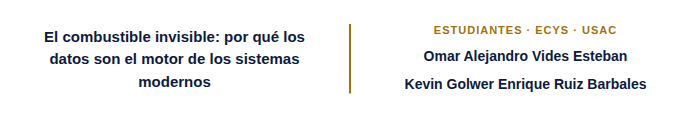
\includegraphics[width=1\linewidth]{labels/pareja52} \end{center}

\textbf{Palabras clave:} datos, sistemas modernos, inteligencia artificial, toma de decisiones, arquitectura de datos.

\begin {multicols}{2}

\section{Introducción}\label{introducciuxf3n-12}

A inicios de 2026, la cantidad de datos generados por la humanidad había superado todas las estimaciones realizadas una década antes. IDC estima que el mundo alcanzará los 175 zettabytes de información a mediados de siglo, cifra que seguirá creciendo con la proliferación de dispositivos, plataformas digitales y sistemas de inteligencia artificial generativa. Los sistemas, en los distintos sectores, dependen del flujo constante de datos para funcionar, adaptarse y mejorar.

Este artículo estudia por qué los datos se han convertido en el recurso central de los sistemas modernos, cómo se procesan y las consecuencias de su gestión adecuada e inadecuada. Este análisis se realiza desde una perspectiva de la ingeniería de sistemas, reconociendo que el diseño de una arquitectura basada en datos no es opcional, sino una prioridad fundamental y un principio básico para los ingenieros del siglo XXI.

\section{Desarrollo}\label{desarrollo-4}

\textbf{¿Qué significa que un sistema sea impulsado por datos?}

Un sistema impulsado por datos (\emph{data-driven system}) es aquel cuyo comportamiento, decisiones y predicciones dependen directamente de la información que recibe y procesa. A diferencia de los sistemas basados en reglas fijas programadas por ingenieros, los sistemas modernos aprenden y se ajustan con base en patrones extraídos de grandes volúmenes de datos. Esto abarca desde motores de recomendación como los de Netflix o Spotify hasta sistemas de detección de fraudes en entidades bancarias guatemaltecas, donde el análisis de transacciones en tiempo real determina si una operación es aprobada o bloqueada.

Este cambio de perspectiva demuestra que la calidad de los datos es tan importante como la calidad del código. Los datos inexactos, duplicados o incompletos pueden dar lugar a decisiones erróneas, pérdidas financieras o interrupciones operativas. Asimismo, campos como la gobernanza de datos, la ingeniería de datos y el control de calidad de la información están cobrando cada vez más importancia dentro de los equipos que intervienen en la toma de decisiones.

\textbf{La arquitectura que sostiene los datos modernos}

Para que los datos sean útiles, deben pasar por una arquitectura diseñada para recopilarlos, almacenarlos, transformarlos y publicarlos de manera confiable. Las arquitecturas modernas de datos incluyen componentes como los \emph{data lakes}, los \emph{data warehouses} y los \emph{pipelines} de procesamiento en tiempo real. Herramientas como Apache Kafka permiten manejar millones de eventos por segundo. Su adopción no se limita a las grandes corporaciones; organizaciones medianas e instituciones públicas en países como Guatemala han incorporado progresivamente estas tecnologías en sus operaciones.

\end {multicols}

\begin{longtable}[]{@{}
  >{\raggedright\arraybackslash}p{(\linewidth - 4\tabcolsep) * \real{0.3333}}
  >{\raggedright\arraybackslash}p{(\linewidth - 4\tabcolsep) * \real{0.3333}}
  >{\raggedright\arraybackslash}p{(\linewidth - 4\tabcolsep) * \real{0.3333}}@{}}
\toprule\noalign{}
\begin{minipage}[b]{\linewidth}\raggedright
Tecnología
\end{minipage} & \begin{minipage}[b]{\linewidth}\raggedright
Función principal
\end{minipage} & \begin{minipage}[b]{\linewidth}\raggedright
Ejemplo de uso
\end{minipage} \\
\midrule\noalign{}
\endhead
\bottomrule\noalign{}
\endlastfoot
Data Lake & Almacenamiento masivo de datos en crudo & Repositorios de logs e imágenes \\
Data Warehouse & Almacenamiento estructurado para análisis & Reportes financieros y BI corporativo \\
Apache Kafka & Streaming de eventos en tiempo real & Detección de fraude bancario en tiempo real \\
Apache Spark & Procesamiento distribuido de grandes volúmenes & Transformación de datos a escala en pipelines ETL \\
Data Mesh & Gestión descentralizada por dominio & Equipos de dominio que publican sus propios datos \\
\end{longtable}

\emph{Tabla 1. Tecnologías clave en arquitecturas modernas de datos. Fuente: Elaboración propia.}

\begin {multicols}{2}

El concepto de \emph{data mesh} ha nacido en la actualidad como alternativa a los modelos centralizados. En lugar de recopilar todos los datos en un único lugar de almacenamiento gestionado por equipos especializados, el \emph{data mesh} propone que cada ámbito empresarial gestione sus propios datos como un producto. El objetivo de este enfoque descentralizado es aumentar las capacidades analíticas sin crear pasos adicionales que ralenticen el proceso.

\textbf{El dato como insumo para la inteligencia artificial}

La inteligencia artificial no puede existir sin datos. Los modelos de \emph{machine learning} son en esencia funciones matemáticas ajustadas a partir de datos pasados. Cuanto mayor sea la calidad de los datos de entrenamiento, mejor será la salida y/o resultados del o los modelos entrenados. Este principio, conocido como \emph{``garbage in, garbage out''}, es una forma contundente de expresar la dependencia que existe entre la IA y la calidad de los datos que la alimentan.

\section{Conclusiones}\label{conclusiones-7}

Los datos ya no son un subproducto de los sistemas, sino que se han convertido en su materia prima principal. La capacidad de los sistemas modernos para aprender, adaptarse y crear valor depende de la disponibilidad, la calidad y la gestión de la información. Esto representa un cambio de perspectiva: ya no basta con crear software que funcione, sino que el diseño debe reconocer que los datos son tan importantes como el código. En el mercado actual se demandan habilidades en materia de gobernanza de datos, arquitectura de canalizaciones y preparación de información para modelos de inteligencia artificial, y las instituciones académicas deberían integrar estas habilidades de forma más completa en sus programas.

\section{Bibliografía}\label{bibliografuxeda-12}

\begin{itemize}
\item
  Reinsel, David, John Gantz, and John Rydning. ``The Digitization of the World: From Edge to Core.'' \emph{IDC White Paper}, November 2018. \url{https://www.seagate.com/files/www-content/our-story/trends/files/idc-seagate-dataage-whitepaper.pdf}.
\item
  Provost, Foster, and Tom Fawcett. \emph{Data Science for Business: What You Need to Know about Data Mining and Data-Analytic Thinking}. Sebastopol, CA: O'Reilly Media, 2013.
\item
  Apache Software Foundation. ``Apache Kafka: A Distributed Streaming Platform.'' \url{https://kafka.apache.org/documentation}.
\item
  Dehghani, Zhamak. \emph{Data Mesh: Delivering Data-Driven Value at Scale}. Sebastopol, CA: O'Reilly Media, 2022.
\end{itemize}

\end {multicols}

\medskip

\suppresschapterfalse

\articletitlecommand
\vspace*{-23mm}
\phantomsection
\label{pareja1}
\addcontentsline{toc}{chapter}{}

\chapter{Modelos de lenguaje en la transformación digital cotidiana}\label{pareja1}

\null\vspace*{-20mm}

\begin{center}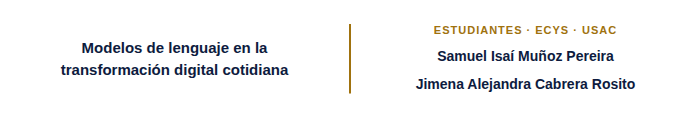
\includegraphics[width=1\linewidth]{labels/pareja1} \end{center}

\begin {multicols}{2}

\textbf{Palabras clave}\\
modelos de lenguaje, inteligencia artificial, vida cotidiana, educación, productividad

\section{Introducción}\label{introducciuxf3n-13}

En pocos años, los modelos de lenguaje se han vuelto parte visible de la transformación digital: ayudan a redactar textos, aclarar dudas y resumir información en cuestión de segundos. Hoy no solo se usan en empresas tecnológicas, sino también por estudiantes, docentes y profesionales en tareas diarias de lectura, escritura y organización.

El objetivo de este artículo es presentar de forma breve cómo estos modelos intervienen en la vida cotidiana, qué beneficios ofrecen y qué riesgos implican si se utilizan sin sentido crítico. De esta manera, se busca aportar elementos para un uso responsable que complemente, y no reemplace, las capacidades humanas.

\section{Artículo}\label{artuxedculo-8}

\textbf{Apoyo en estudio y trabajo}

En el ámbito académico, los modelos de lenguaje se usan para explicar conceptos difíciles, resumir textos largos, proponer ejemplos y ayudar a organizar ideas. Esto puede ahorrar tiempo y hacer más accesible la comprensión de lecturas complejas, siempre y cuando el estudiante revise y confirme la información con otras fuentes.

En el trabajo, se emplean para redactar borradores de correos, informes y presentaciones, así como para mejorar redacción y ortografía. Son útiles para comenzar un texto o ganar claridad, pero requieren revisión final del usuario, ya que los modelos pueden cometer errores o presentar datos inexactos.

\textbf{Uso en la vida cotidiana}

En la vida diaria, estas herramientas se usan para planificar actividades, organizar tareas, generar ideas de proyectos y recibir recomendaciones básicas. Muchas personas las aprovechan para estructurar su día, preparar mensajes o tener sugerencias rápidas sin buscar en múltiples páginas.

También se han integrado en aplicaciones, asistentes virtuales y procesadores de texto, por lo que su presencia pasa a menudo desapercibida. Esto muestra que la transformación digital no solo ocurre en grandes sistemas, sino en pequeñas acciones cotidianas como escribir, preguntar o tomar notas.

\textbf{Beneficios y riesgos}

Entre los principales beneficios se encuentran el ahorro de tiempo, el apoyo a la escritura y el acceso más sencillo a explicaciones sobre temas complejos. Para quienes tienen dificultades para redactar o sintetizar, los modelos pueden servir como guía inicial y como recurso de apoyo.

Sin embargo, un uso acrítico puede generar dependencia, pérdida de práctica en la escritura y aceptación de información incorrecta. Además, al no conocer el origen exacto de todos los datos, es necesario contrastar lo que generan con fuentes confiables y mantener siempre el juicio personal. Como se muestra en la Figura 1, los modelos de lenguaje presentan distintos usos, beneficios y riesgos según el ámbito en que se empleen.

\begin{center}
\includegraphics[width=1\linewidth]{articulos_seleccionados/imagenes_articulos_seleccionados/A_pareja1/p1} \end{center}

\emph{Figura 1: Beneficios, usos y riesgos de los modelos de lenguaje en la vida cotidiana y profesional. Fuente: Elaboración propia.}

\textbf{Uso responsable}

El uso responsable implica ver al modelo de lenguaje como herramienta y no como sustituto del propio pensamiento. En el contexto universitario, esto significa revisar los textos generados, adaptar el contenido al propio estilo, citar las fuentes reales consultadas y no presentar como propio un texto producido automáticamente.

En la vida diaria, también conviene definir límites: aprovechar la ayuda para organizar y redactar, pero mantener decisiones importantes bajo análisis humano. De esta forma, la transformación digital puede apoyar el aprendizaje y la productividad sin debilitar la autonomía ni la responsabilidad personal.

\section{Conclusiones}\label{conclusiones-8}

Los modelos de lenguaje forman ya parte de la vida académica y cotidiana, apoyando tareas de lectura, escritura, organización y comunicación. Bien utilizados, ayudan a ahorrar tiempo, aclarar dudas y estructurar mejor la información que usamos a diario, lo que facilita tanto el aprendizaje como la realización de actividades en distintos contextos. No obstante, su uso exige una actitud crítica: revisar datos, contrastar fuentes y evitar que sustituyan la práctica de escribir y pensar por cuenta propia. Solo así podrán contribuir positivamente a la transformación digital sin afectar el desarrollo de habilidades fundamentales en el estudio y el trabajo.

\section{Bibliografía}\label{bibliografuxeda-13}

\begin{itemize}
\item
  Adoption of Large Language Model AI Tools in Everyday Tasks. 2025. \emph{Journal of Medical Internet Research} 27.
\item
  Evidently AI. 2025. 55 Real-World LLM Applications and Use Cases from Top Companies.
\item
  RoAI Institute. 2024. How Generative AI Is Transforming Our Daily Lives.
\end{itemize}

\end {multicols}

\medskip

\suppresschapterfalse
\clearpage
\suppressbackgroundtrue

\includepdf[pages=1,fitpaper=true]{articulos_seleccionados/images/seccion4.pdf}
\suppressbackgroundfalse

\articletitleafterpdfsection
\phantomsection
\label{pareja36}
\addcontentsline{toc}{chapter}{}

\chapter{Cuando la nube se vuelve vulnerable: desafíos de seguridad en la infraestructura digital moderna}\label{pareja36}

\null\vspace*{-20mm}

\begin{center}
\includegraphics[width=1\linewidth]{labels/pareja36} \end{center}

\textbf{Palabras clave:} ciberseguridad, computación en la nube, gobernanza digital, protección de datos, infraestructura tecnológica.

\begin {multicols}{2}

\section{Introducción}\label{introducciuxf3n-14}

La computación en la nube se ha convertido en algo fundamental en la transformación digital. Hoy en día, desde pequeños sistemas hasta grandes corporaciones dependen de las infraestructuras remotas para almacenar datos, ejecutar aplicaciones y ofrecer servicios en tiempo real. La nube representa mucha agilidad, escalabilidad y eficiencia a un costo razonable; el problema es que está abierta a nuevos escenarios de riesgos.

Hablar de seguridad en la nube implica reconocer que la protección de la información no depende únicamente de servidores físicos. La infraestructura digital moderna es distribuida, dinámica y se ha logrado la correcta interconexión entre servicios. Hoy en día los desafíos actuales no son solo técnicos sino también estratégicos y éticos. Analizar vulnerabilidades permite comprender la importancia de fortalecer la gobernanza y la cultura de seguridad.

\section{Desarrollo}\label{desarrollo-5}

Uno de los principales desafíos en entornos de la nube es el modelo de responsabilidad compartida. Aunque los proveedores ofrecen mecanismos avanzados de protección, la configuración y gestión de los datos continúa siendo responsabilidad del usuario. Muchas brechas de seguridad no se originan por fallos en la infraestructura del proveedor, sino por errores humanos, permisos mal configurados o credenciales comprometidas. Esta realidad evidencia que la tecnología, por sí sola, no garantiza protección.

La infraestructura digital moderna se caracteriza por su interconectividad. Microservicios, APIs y contenedores permiten mayor flexibilidad, pero también amplían la superficie de ataque. Un solo punto vulnerable puede comprometer múltiples sistemas interrelacionados. Según el National Institute of Standards and Technology (NIST), la gestión del riesgo en infraestructuras críticas requiere un enfoque integral que combine controles técnicos, monitoreo constante y evaluación continua de amenazas.

\begin{center}
\includegraphics[width=0.8\linewidth]{articulos_seleccionados/imagenes_articulos_seleccionados/A_pareja36/p1} \end{center}

\emph{Figura 1. Vulnerabilidades y riesgos en modelos de servicio en la nube (IaaS, PaaS y SaaS). Fuente: ResearchGate, 2024.}

El análisis comparativo de los modelos de servicio en la nube permite identificar cómo varían los riesgos según el nivel de responsabilidad del usuario. IaaS presenta vulnerabilidades asociadas a la infraestructura, PaaS a dependencias y APIs, y SaaS a configuraciones de acceso. Asimismo, se evidencian diferencias en los costos de brechas y en las tasas de mitigación, lo que demuestra que la seguridad no es uniforme y requiere estrategias específicas según el modelo adoptado.

Otro reto relevante es la evolución constante de los ciberataques. El ransomware ha pasado de ser un ataque aislado a convertirse en una estrategia organizada que busca paralizar servicios completos. En entornos de nube, donde grandes volúmenes de información se concentran en plataformas accesibles remotamente, el impacto puede ser significativo. Esto exige implementar cifrado robusto, autenticación multifactor y políticas estrictas de control de acceso.

Desde la perspectiva de la gobernanza, la protección de datos personales representa un compromiso ético y legal. Las organizaciones deben garantizar confidencialidad, integridad y disponibilidad de la información. La European Union Agency for Cybersecurity (ENISA) destaca que la seguridad en la nube debe integrarse desde el diseño del sistema y no como una medida posterior. Esto implica que los ingenieros en sistemas asuman un rol activo en la planificación de arquitecturas seguras y sostenibles.

La capacitación del personal, la actualización constante y la concientización sobre amenazas digitales son elementos esenciales para reducir riesgos. La nube puede ser altamente segura si existe una estrategia clara, pero se vuelve vulnerable cuando se descuida la gestión interna y la supervisión continua.

\section{Conclusiones}\label{conclusiones-9}

La infraestructura digital moderna ofrece enormes ventajas en términos de innovación y eficiencia, pero también plantea desafíos de seguridad que no pueden ignorarse. La nube no es inherentemente insegura; su vulnerabilidad surge cuando se subestiman los riesgos asociados a su gestión y configuración.

En el ámbito de la Ingeniería en Sistemas, estos desafíos exigen una visión integral que combine conocimiento técnico, capacidad de análisis y responsabilidad ética. La gobernanza en entornos digitales debe fortalecerse mediante políticas claras, monitoreo constante y formación continua. Proteger la información en la nube no es solo una tarea técnica, sino un compromiso profesional. Además, es fundamental adoptar estrategias proactivas de seguridad que permitan anticipar y mitigar amenazas en entornos digitales cada vez más complejos.

\section{Bibliografía}\label{bibliografuxeda-14}

\begin{itemize}
\item
  Cloud Security Alliance. \emph{Security Guidance for Critical Areas of Focus in Cloud Computing}. Version 4.0. New York: Cloud Security Alliance, 2017.
\item
  European Union Agency for Cybersecurity (ENISA). \emph{Cloud Security for SMEs}. Luxembourg: Publications Office of the European Union, 2015.
\item
  National Institute of Standards and Technology (NIST). \emph{Framework for Improving Critical Infrastructure Cybersecurity}. Version 1.1. Gaithersburg, MD: NIST, 2018.
\item
  Cloud Security Risks and Mitigation Strategies: A Review of Current Trends and Future Directions. ResearchGate, 2024. \url{https://www.researchgate.net/publication/395648103}
\end{itemize}

\end {multicols}

\medskip

\suppresschapterfalse

\articletitlecommand
\vspace*{-23mm}
\phantomsection
\label{pareja17}
\addcontentsline{toc}{chapter}{}

\chapter{El valor de tus datos: el precio de la privacidad}\label{pareja17}

\null\vspace*{-20mm}

\begin{center}
\includegraphics[width=1\linewidth]{labels/pareja17} \end{center}

\begin {multicols}{2}

\textbf{Palabras clave}\\
datos personales, privacidad de la información, data brokers, publicidad dirigida

\section{Introducción}\label{introducciuxf3n-15}

Muchas veces, cuando se habla del valor de los datos, se piensa únicamente en información como números de tarjetas de crédito o datos sensibles. Sin embargo, en el entorno digital su valor va más allá de eso. Cada interacción, cada ``me gusta'' y cada actividad dentro de internet produce datos relevantes para empresas y campañas de marketing. En la actualidad, los datos personales representan un activo de gran valor (Federal Trade Commission 2014).

A partir de esos datos, se construyen perfiles que permiten segmentar contenido y orientar publicidad. Julie Brill advierte que estos perfiles pueden basarse en información incompleta o errónea, afectando directamente el trato que recibe el usuario. El problema no se limita solo a la recolección de datos, sino también a la falta de transparencia sobre cómo se procesan, circulan y utilizan dentro del ecosistema digital.

\section{Artículo}\label{artuxedculo-9}

\textbf{Recolección de datos en el entorno digital}

La información suele obtenerse a través de registros e interacciones en redes sociales, del contenido que consumimos, de lo que buscamos y en general, de toda nuestra actividad en distintas plataformas.

Un estudio realizado en 2023 sobre la venta de información del personal militar estadounidense evidenció un mercado dedicado a la comercialización de datos de ubicación. En esta investigación, 2 de los 12 brokers investigados se dedicaban exclusivamente a la venta de información locacional obtenida a través de aplicaciones móviles (Sherman et al.~2023).

Una de las técnicas principales del rastreo web es la sincronización de cookies, en donde la información de seguimiento se intercambia directamente entre sitios. Esto permite un rastreo amplio y la unión de distintos perfiles digitales. Cuando este tipo de rastreo es bloqueado, existe el fingerprinting, una técnica enfocada en obtener información sobre el dispositivo como hardware, sistema operativo y el navegador (Englehardt and Narayanan 2016).

\textbf{Comercialización y circulación de la información personal}

Los datos no se quedan únicamente en la plataforma donde fueron generados, sino que pasan a formar parte de una red más amplia. Actualmente, este entorno es una industria multimillonaria basada en la obtención, clasificación y venta de datos y perfiles de usuarios.

La Federal Trade Commission explica que los data brokers obtienen información personal de diversas fuentes y la utilizan para fines como marketing, validar la identidad y detectar fraudes. Como estas empresas generalmente no tienen contacto directo con el público, muchas personas no saben qué datos se están guardando sobre ellas, ni cómo se usan (Federal Trade Commission 2014).

\textbf{Usos y fines del perfilado de datos}

Los data brokers no solo venden datos individuales, sino también grupos y categorías que las empresas pueden usar para lanzar campañas, personalizar ofertas o identificar públicos con ciertas características. Por ejemplo, una categoría como ``Biker Enthusiasts'' puede servirle a una empresa de motocicletas para ofrecer cupones, pero también puede servirle a una compañía de seguros para excluir a esos clientes (Federal Trade Commission 2014).

Cuando los datos se cruzan de forma constante para crear perfiles, también pueden hacer funcionar sistemas automáticos que organizan, seleccionan o personalizan lo que una persona ve, recibe e incluso la forma en que es tratada dentro de un servicio o aplicación digital. Como se muestra en la Figura 1, el ciclo de circulación abarca desde la recolección hasta los usos comerciales e institucionales.

\begin{center}
\includegraphics[width=0.8\linewidth]{articulos_seleccionados/imagenes_articulos_seleccionados/A_pareja17/p1} \end{center}

\emph{Figura 1: Ciclo de circulación y aprovechamiento de datos personales en el ecosistema digital. Fuente: Elaboración propia.}

\section{Conclusión}\label{conclusiuxf3n-5}

La obtención y venta de los datos personales es uno de los principales recursos de la economía digital actual. Sin embargo, el problema de privacidad no está solo en que esta información se recoja, sino en que circule con poco seguimiento entre distintos grupos, lo que dificulta saber quién accede a ella, cómo la obtiene y para qué la utiliza. Es importante como usuarios ser conscientes del valor y uso de nuestros datos. Comprender que nuestros datos son compartidos y nuestra publicidad está dirigida.

\section{Bibliografía}\label{bibliografuxeda-15}

\begin{itemize}
\item
  Englehardt, Steven, and Arvind Narayanan. 2016. \emph{Online Tracking: A 1-Million-Site Measurement and Analysis.}
  \url{https://senglehardt.com/papers/ccs16_online_tracking.pdf}
\item
  Federal Trade Commission. 2014. \emph{Data Brokers: A Call for Transparency and Accountability.} \url{https://www.ftc.gov/system/files/documents/reports/data-brokers-call-transparency-accountability-report-federal-trade-commission-may-2014/140527databrokerreport.pdf}
\item
  Sherman, Justin, et al.~2023. \emph{Data Brokers and the Sale of Data on U.S. Military Personnel.} Duke University.
\end{itemize}

\end {multicols}

\medskip

\suppresschapterfalse

\articletitlecommand
\vspace*{-23mm}
\phantomsection
\label{pareja59}
\addcontentsline{toc}{chapter}{}

\chapter{Guatemala ante la IA: estudiantes avanzan, el país se rezaga}\label{pareja59}

\null\vspace*{-20mm}

\begin{center}
\includegraphics[width=1\linewidth]{labels/pareja59} \end{center}

\textbf{Palabras clave:} inteligencia artificial, estudiantes universitarios, empleabilidad, brecha tecnológica, Guatemala.

\begin {multicols}{2}

\section{Introducción}\label{introducciuxf3n-16}

En la actualidad, es casi imposible hablar de Ingeniería en Sistemas sin mencionar la inteligencia artificial. La IA ya no es solo una proyección del futuro, sino una herramienta de uso cotidiano para estudiar, programar, investigar, resumir textos o generar ideas para proyectos. Su uso se ha vuelto cada vez más frecuente en los procesos de aprendizaje y en la formación técnica de los estudiantes.

En Guatemala, muchos estudiantes ya la han adoptado como parte de su rutina académica. Sin embargo, mientras ellos avanzan con rapidez, el país no parece ir al mismo ritmo. Diversos reportes muestran que Guatemala todavía presenta rezagos importantes en el desarrollo de la inteligencia artificial y no cuenta con una implementación sólida a nivel nacional.

\section{Desarrollo}\label{desarrollo-6}

\textbf{La IA como parte de la vida universitaria}

Muchos estudiantes usan herramientas de IA para comprender mejor un tema, mejorar su código, practicar entrevistas técnicas o incluso aprender nuevas tecnologías. Ya no se trata solo de reproducir información, sino de contar con un apoyo constante para el aprendizaje.

Además, varias universidades en Guatemala han comenzado a incluir cursos, diplomados e incluso maestrías relacionadas con inteligencia artificial, ciencia de datos y automatización. Esto demuestra que existe un esfuerzo por actualizar la formación profesional.

\textbf{El rezago del país: el verdadero desafío}

El Programa de las Naciones Unidas para el Desarrollo (PNUD) señala que Guatemala enfrenta limitaciones en infraestructura tecnológica, inversión, regulación y desarrollo de talento especializado en IA. Esto indica que, aunque existe interés, todavía no hay un ecosistema sólido que impulse la inteligencia artificial a gran escala.

Por otro lado, el \emph{Global Skills Report 2025} de Coursera ubica a Guatemala en posiciones bajas en rankings de habilidades tecnológicas dentro de América Latina. Esto refleja que el país aún está lejos de competir con economías más avanzadas en este campo.

\begin{center}
\includegraphics[width=0.8\linewidth]{articulos_seleccionados/imagenes_articulos_seleccionados/A_pareja59/p1} \end{center}

\emph{Ilustración 1. Ranking regional de habilidades y madurez en IA en América Latina y el Caribe. Fuente: Coursera, Global Skills Report 2025, p.~43.}

\begin{center}
\includegraphics[width=0.8\linewidth]{articulos_seleccionados/imagenes_articulos_seleccionados/A_pareja59/p2} \end{center}

\emph{Ilustración 2. Resultados por pilar de la Evaluación del Panorama de la Inteligencia Artificial en Guatemala (AILA). Fuente: Programa de las Naciones Unidas para el Desarrollo (PNUD), ``Guatemala avanza hacia un uso inclusivo, responsable y transformador de la Inteligencia Artificial'', 28 de noviembre de 2025.}

\textbf{El futuro laboral}

Si Guatemala no acelera su desarrollo en IA, muchas empresas locales podrían quedarse atrás frente a la competencia internacional; los profesionales mejor preparados podrían buscar oportunidades fuera del país o trabajar de forma remota para empresas extranjeras, y se ampliaría la brecha entre quienes dominan la IA y quienes no.

Si los estudiantes actuales logran formarse bien en IA, automatización y análisis de datos, pueden convertirse en el motor que impulse la transformación digital del país. En lugar de esperar que el cambio provenga solo de las instituciones, este también puede surgir del talento joven.

El futuro laboral del ingeniero en sistemas en Guatemala dependerá en gran medida de su capacidad de adaptación. Ya no basta con saber programar; ahora es clave integrar IA, automatizar procesos y entender cómo usar estas herramientas de manera ética y estratégica.

\section{Conclusiones}\label{conclusiones-10}

La inteligencia artificial ya forma parte de la formación universitaria en Guatemala. Los estudiantes la están adoptando rápidamente y las universidades comienzan a actualizar sus programas. Sin embargo, los informes muestran que el país aún enfrenta un rezago importante en el desarrollo e implementación de IA. Esto impacta directamente el futuro laboral del ingeniero en sistemas. Si el ecosistema nacional no crece al mismo ritmo que la formación académica, el talento podría migrar o limitarse a trabajar para mercados externos. El reto no es solo aprender IA, sino lograr que Guatemala también avance, porque no se trata solo de tener estudiantes preparados, sino de tener un país preparado para aprovechar ese talento.

\section{Bibliografía}\label{bibliografuxeda-16}

\begin{itemize}
\item
  Programa de las Naciones Unidas para el Desarrollo. ``Guatemala avanza hacia un uso inclusivo, responsable y transformador de la Inteligencia Artificial.'' 28 de noviembre de 2025.
\item
  Coursera. \emph{Global Skills Report 2025}. 2025.
\item
  Weinar, Agnieszka, y Amparo Klekowski von Koppenfels. ``Migración altamente cualificada: concepto y definiciones.'' En \emph{Migración altamente cualificada: Entre el asentamiento y la movilidad}. Cham: Springer, 2020.
\end{itemize}

\end {multicols}

\medskip

\suppresschapterfalse

\articletitlecommand
\vspace*{-23mm}
\phantomsection
\label{pareja40}
\addcontentsline{toc}{chapter}{}

\chapter{Cuando el software hiere: el deber ético del ingeniero ante la información sensible}\label{pareja40}

\null\vspace*{-20mm}

\begin{center}
\includegraphics[width=1\linewidth]{labels/pareja40} \end{center}

\textbf{Palabras clave:} daño, empatía, datos, usuario, ética.

\begin {multicols}{2}

\section{Introducción}\label{introducciuxf3n-17}

Cuando un ingeniero desarrolla algo nuevo, puede elegir dos caminos: el camino fácil, donde cumplirá su objetivo desapegándose de las consecuencias que tenga tomarlo, y el correcto, que involucra más trabajo pero asegura una mejor integridad para el usuario final. Un ingeniero debe caracterizarse no solamente por sus habilidades técnicas, sino también por sus habilidades blandas.

Existen una gran variedad de casos en los que se ha visto cómo una decisión tomada por los ingenieros a cargo de desarrollar un sistema, o bien la omisión de un potencial problema, puede desencadenar una cadena de eventos que pueden ser altamente perjudiciales para los usuarios finales. Por lo general las noticias que cubren estos casos hablan únicamente de números, pero no del daño provocado a los usuarios afectados.

\section{Desarrollo}\label{desarrollo-7}

El código de ética de la ACM establece el daño como cualquier consecuencia negativa e incluye la divulgación injustificada de información entre los ejemplos del mismo. Basándonos en esta definición, un ingeniero en sistemas es capaz de injuriar a otra persona debido a la falta de empatía y responsabilidad en el desarrollo de aplicaciones, reflejándose en varios casos que han sucedido durante la última década.

Como un claro ejemplo de una infracción al código de ética mencionado anteriormente, podemos mencionar lo sucedido en México el pasado 9 de enero, debido a la nueva ley que se aprobó: los usuarios de líneas telefónicas deben de vincular sus líneas a una persona física o moral. Debido a la naturaleza del trámite, se requiere información personal de los ciudadanos. La compañía Telcel desarrolló un sistema que le permite a sus usuarios realizar el registro de forma virtual; al recolectar la información necesaria de los usuarios quedaba completado el registro. El problema sucedió que al tener el registro en operación, Telcel permitió el ingreso de cualquier número celular y el sistema presuntamente retornaba los datos almacenados de la persona ---que incluye información sensible como el nombre completo, información fiscal y el correo electrónico--- sin la debida verificación y autenticación previa.

Cuando una persona ingresa sus datos en cualquier plataforma, generalmente lo llegamos a ver como un simple registro, algo que es necesario. Nosotros como ingenieros en sistemas debemos ponernos en el lugar de los usuarios que depositan su confianza indirectamente en nosotros. Debemos empezar a ver a las personas que están detrás de esos datos registrados en nuestro repositorio de datos, y el daño que podemos causarles, sin necesidad de tener un contacto con ellas.

Una simple exposición innecesaria de un número telefónico puede escalar a una suplantación de identidad o un robo de cuentas bancarias. ¿Acaso esto no entra en la definición de daño planteada por la ACM? Nosotros como ingenieros en sistemas debemos de ser conscientes de que, a pesar de que pueda o no pertenecer a la jurisdicción en la que ejercemos, las guías y pautas para un desarrollo responsable sí existen; es solo cuestión de seguirlas, a pesar de las dificultades en desarrollo y diseño que estas puedan conllevar.

\end {multicols}

\begin{longtable}[]{@{}ll@{}}
\toprule\noalign{}
Entidad & Normativo \\
\midrule\noalign{}
\endhead
\bottomrule\noalign{}
\endlastfoot
ACM & Code of Ethics and Professional Conduct \\
GDPR & Principles relating to processing of personal data \\
IEEE & Code of Ethics \\
\end{longtable}

\emph{Tabla 1. Entidades y sus respectivos normativos de ética y/o protección de datos. Fuente: Elaboración propia.}

\begin {multicols}{2}

Debemos de empezar a concebir las nuevas formas de dañar personas que se han desarrollado en una era en constante cambio, donde la comodidad se hace cada vez más accesible, y concientizarnos del deber intrínseco que se ha vuelto parte de nuestra labor profesional.

\section{Conclusiones}\label{conclusiones-11}

En la era digital donde nos encontramos, debemos comprender que nuestras decisiones durante el desarrollo pueden causar un daño irreparable a todos los usuarios, que no se traduce a una lesión física, y que puede cambiar por completo la vida de los afectados. Al aceptar esta labor, debemos de entender la magnitud de nuestro deber moral, el cual es seguir los lineamientos ya establecidos por las entidades encargadas de informar a todos los profesionales del campo, y establecer una serie de principios liderados por la empatía, responsabilidad y honestidad absoluta que nos permitan algún día llegar a un punto en el que no le hagamos daño a las personas. Como futuros profesionales, nosotros mismos quisiéramos incitar a cada uno de nuestros colegas a siempre preguntarse esto al momento de trabajar en un sistema: ¿cómo esta implementación podría causarle daño a alguien más?

\section{Bibliografía}\label{bibliografuxeda-17}

\begin{itemize}
\item
  Association for Computing Machinery. ``ACM Code of Ethics and Professional Conduct.'' \url{https://www.acm.org/code-of-ethics}.
\item
  General Data Protection Regulation. ``Art. 5 GDPR - Principles relating to processing of personal data.'' \url{https://gdpr-info.eu/art-5-gdpr/}.
\item
  Institute of Electrical and Electronics Engineers. ``IEEE Code of Ethics.'' \url{https://www.ieee.org/about/corporate/governance/p7-8.html}.
\item
  Nares, Obed. ``Telcel filtra datos personales de usuarios en México: el registro de líneas celulares falla en sus primeros días.'' \emph{Xataka México}, 12 de enero de 2026. \url{https://www.xataka.com.mx/telecomunicaciones/telcel-filtra-datos-personales-usuario-mexico-registro-lineas-celulares-falla-sus-primeros-dias}.
\end{itemize}

\end {multicols}

\medskip

\suppresschapterfalse

\bibliography{book.bib,packages.bib}

%%%%\printindex
\clearpage
\suppressbackgroundtrue

\includepdf[pages=1,fitpaper=true,noautoscale=false]{articulos_seleccionados/images/contraportada.pdf}
\suppressbackgroundfalse


\end{document}
